%\documentclass[DIV19]{scrartcl}
%\usepackage[paper size={90mm, 120mm},left=2mm,right=2mm,top=2mm,bottom=2mm,nohead]{geometry}
% FIXME try prettyref
\documentclass[oneside,a4paper,12pt,BCOR20mm,DIV14]{scrbook} % should be DIV14
%\documentclass{book}
% this gives a bit more than 2cm margin right and 4cm left
% koma-script.pdf: A4 is 210mmx297mm, BCOR is substraced before the page
% width is divided into DIV parts (HLU), a one sided leaves 1.5 HLU
% HLU*DIV=210-BCOR -> DIV=(210-BCOR)/HLU
% I want BCOR= 20mm 1.5 HLU = 20 mm 
% -> DIV=truncate(190*1.5/20) = truncate(14.25)=14
% I could use headinclude so that the header isn't printed into the margin

% Initially two softbound theses should be submitted to the
% Examinations Office for the examiners. Softbound theses should have
% the pages glued in.
% They don't need gold lettering on the spine.

%\includeonly{spatio-angular}

\usepackage[utf8]{inputenc}
%\usepackage[T1]{fontenc}
\usepackage[usenames,dvipsnames]{color}
\usepackage[onehalfspacing]{setspace} 
\usepackage{graphicx}
\usepackage{longtable}
\usepackage{float}
\usepackage{wrapfig}
\usepackage{soul}
\usepackage{amssymb}
\usepackage{amsmath}

\usepackage{pdfcomment}

% choose font here: http://www.tug.dk/FontCatalogue/mathfonts.html
%\usepackage[math]{iwona}
\usepackage[math]{kurier}
%\usepackage{cmbright}
\usepackage[T1]{fontenc}

\usepackage[hypertex,breaklinks]{hyperref} % breaklinks only seems to
                                           % work with dvipdfm,
                                           % otherwise urls have no
                                           % line breaks
\usepackage{units}
\usepackage[disable]{todonotes} % for draft, disable for final
\usepackage{refcheck} % for draft, uncomment for final
\usepackage{lineno}
\usepackage{nomencl}
%\special{background Black}\special{color Green}
%\usepackage[utf8x]{inputenc} 
%\usepackage[T2A]{fontenc} % for the russian reference
\usepackage{wasysym} %diameter
% http://www.andy-roberts.net/misc/latex/latextutorial3.html

%\usepackage{url} % natbib.pdf p.11 break urls up, seems to be done
                 % with hyperref, though

\usepackage{natbib}


% for app_hilo
\usepackage{listings}
\usepackage{color}
\usepackage{textcomp}
\usepackage{subfigure}


% \listfiles % show which files are loaded by tex

\bibpunct{(}{)}{;}{a}{}{,}
\makenomenclature
\newcommand{\vect}[1]{\mathbf{#1}}
\renewcommand{\r}{\vect r}
\renewcommand{\a}{\vect a}
\newcommand{\s}{\vect s}
\def\k{\vect k}
\def\d{\vect d}
\def\e{\vect e}
\def\f{\vect f}
\def\c{\vect c}
\def\x{\vect x}
\def\y{\vect y}
\def\z{\vect z}
\def\q{\vect q}
\def\p{\vect p}
\def\l{\vect l}

\newcommand{\nvect}[1]{\vect{\hat{#1}}}
%\renewcommand{\i}{\nvect i}
\newcommand{\vi}{\nvect \i}
\def\hc{\nvect c}
\def\hs{\nvect s}
\def\hd{\nvect d}
\def\hx{\nvect x}
\def\hy{\nvect y}

\def\hz{\nvect z}
\def\n{\nvect n}
\def\t{\nvect t}
\def\m{\nvect m}
\def\vrho{\boldsymbol\rho}
\def\abs#1{\mathopen| #1 \mathclose|}


\renewcommand{\O}{\textsf{O}} % oxygen

% conclusions of paragraphs in the margin
%\usepackage[marginparwidth=2.5cm]{geometry}
\setlength{\marginparwidth}{2.5\marginparwidth}
\reversemarginpar
\newcommand{\cm}[1]{\marginpar{\small #1}}
% include eps or pdf file, that was generated by inkscape, depending
% on if pdflatex or latex processes this file. latex allows a faster
% development cycle but pdflatex generates a smaller and better final
% pdf output
\def\svgending{\ifx\pdfoutput\undefined% 
  .eps_tex% 
  \else%
  .pdf_tex%
  \fi}

% use \svginput{1}{bla} to include bla.svg, make sure you keep this in
% one line, so that make can automatically find the dependencies with
% sed
\newcommand{\svginput}[2]{{\def\svgscale{#1}\input{#2\svgending}}}

\def\pdfending{\ifx\pdfoutput\undefined% 
  .vector.eps% 
  \else%
  .vector%
  \fi}
\newcommand{\pdfinput}[2]{\includegraphics[width=#1]{#2\pdfending}}

% example call \imagw{8cm}{bla.jpg}{bla}{caption abl}
\newcommand{\imagw}[4]{
  \begin{figure}[!hbt]
    \centering
    \includegraphics[width=#1]{#2}
    \caption{#4}
    \label{fig:#3}
  \end{figure}
}

\def\jpgending{\ifx\pdfoutput\undefined% 
  .eps% 
  \else%
  %
  \fi}
% use like this \jpginput{8cm}{imagefile}{caption ...  make sure all
% characters until the opening brace for the caption are on one line
\newcommand{\jpginput}[3]{\imagw{#1}{#2\jpgending}{#2}{#3}}

% this is for plots that are generated by gnuplot
\newcommand{\gnuplotinput}[2]{\begin{figure}[!hbt]
    \centering
    \includegraphics{#1_gnuplot}
    \caption{#2}
    \label{fig:#1}
  \end{figure}}

\newcommand{\celegans}{\emph{C.~elegans}}
\DeclareMathOperator{\sign}{sign}
\DeclareMathOperator*{\sinc}{sinc}

% reference to picture
\newcommand{\figref}[1]{\figurename~\ref{#1}}
\title{Spatio-angular microscope} % i don't call make title
\author{Martin Kielhorn}
% short summary at the beginning of a section
\newenvironment{summary}{\begin{quote}\small}{\end{quote}}

\begin{document}
\listoftodos
%\linenumbers
\begin{titlepage}
  
  \hspace{-4cm}
  \svginput{1}{objective-trace}



  \vspace{-5cm}
  
  \hspace{4cm}\textsf{\Huge Spatio--Angular Microscopy}
  
  \vspace{2cm}
  \hspace{6cm}\textsf{\huge PhD Thesis}


  \vspace{3cm}
  \hspace{4cm}\textsf{\Large Martin Kielhorn}
  
  \vspace{1cm}
  \hspace{4cm}\textsf{\Large July 2012}
\end{titlepage}
\newpage
\include{abstract}
\urlstyle{sf}
%\setcounter{tocdepth}{3}
\section*{Preface}
\begin{flushright}
  M.~K.
\end{flushright}

\noindent
Jena, Germany

\noindent
July 2012

\newpage
\tableofcontents
\printnomenclature
\chapter{Introduction}
\label{sec:intro}
\begin{summary}
  In this work I discuss a modification of a fluorescence microscope    \cma{my device}
  that minimizes the toxic effects of the excitation light.

  In the following introductory chapter I describe what phototoxicity   \cma{phototoxicity}
  is and how it comes about. Then I give an example of how it
  influences biological observations in a developing \celegans\ 
  embryo and describe how this particular biological system can be
  used to evaluate and compare the phototoxicity of different microscopes.

  Later in this chapter I give an overview of image formation   \cma{cameras}
  in the wide-field microscope and I describe its principle limitations
  regarding resolution and depth discrimination. Furthermore, I
  discuss the two most important current image detector technologies
  --- electron multiplying charge-coupled devices (EMCCD) and
  scientifc complementary metal–oxide–semiconductor (sCMOS).
\end{summary}
\nomenclature{EM-CCD}{Electron multiplying charge-coupled devices}
Regardless of whether it is the picture of earth captured by an
orbiting satellite, the x-ray motion picture of a running dog or the
time-lapse recording of a blooming flower. Images capture our
imagination and they are a good starting point to develop new models
and theories.

This is particularly true for microscopy.  Only after people became
aware of microorganisms by direct observation, medieval quack could
finally be overcome and modern medicine based on the scientific
method flourished instead.

Even today --- with electron microscopes, magnetic resonance
tomography and sequencing machines --- optical microscopy still is an
indispensable tool for research of living organisms.

Fluorescence microscopy is of particular importance: It enables the     \cma{labelling, switching}
scientist to selectively label a particular type of molecule in living cells
and observe how they perform their biological function.

Besides localizing molecules it is possible to measure physical
quantities inside of the sample. There are, for example, fluorescent
labels that report membrane potentials or viscosity inside of cells.

Finally, it is even possible to exert a controlling function with the
excitation light: There are compounds that locally release chemicals
when illuminated and there are  genetically encoded ion channels that can be
switched by light \citep{Boyden2005}.

However, the excitation light introduces unnatural and potentially
deleterious energy into the specimen. If the exogenous light harms the
observed organism in any way, this effect is called phototoxicity.

% dennoch: from photophysical prospective of single- and multi-photon
% microcopy, probably the most disheartening reality is the occurrence
% of photobleaching and photodamage
% \citep{diaspro2009nanoscopy}

There are a number of techniques that can reduce phototoxicity: Two
photon excitation, controlled light exposure, selective plane
illumination, highly inclined and laminated optical sheet, and oblique
plane microscopy. I introduce them in
chapter \ref{sec:approaches}. These techniques have different
pros and cons and not all are equally suited for a specific problem,
e.g.\ selective plane illumination is very effective, but it needs two
perpendicular lenses and can not be used for multiwell plates or to
observe the liver of a living, adult mouse.

In this work I present an approach that makes use of modern display
and camera technology. We only modify the microscope's illumination
path, the space around objective lens and specimen remains as
accessible as in any conventional wide-field microscope.



\section{Phototoxicity in life sciences and the model organism
  \celegans}
\label{sec:intro-phototoxicity}
The partner in our project who is responsible for decisions related to
life sciences and biology is Institut Pasteur (Paris, FR). They work
on infectious diseases. 

In order to motivate the importance of phototoxicity, I would like to
portray an elegant drug screening experiment which I have seen on one
of my visits in Paris: An automatic microscope continuously images a
cell culture in multiwell plates. These cells carry a pathogen. The
pathogen, the nuclei of the cultured cells and the membranes of the
cells are each stained with a different fluorophore. The cells in each
well of the plates are exposed to a different chemical.

A chemical is considered a hit and will be investigated during further
trials, when the time lapse images show that the culture cells stay
healthy and the number of pathogens decrease. As neither people nor
animals come to harm, this screening experiment is an impeccable
method to systematically understand and hopefully heal certain
diseases. However, this experiment does not work very well, if the
excitation light --- and not the drug --- kills the pathogens. The
effect of phototoxicity should therefore be minimized.


Now one would hardly develop a microscope and directly test it with
dangerous pathogens. As part of our collaboration, the Institut
Pasteur therefore developed a safe biological test system that is
relatively easy to maintain \citep{Stiernagle2006} and allows to test
the phototoxicity of various microscopes \citep{Tinevez2012}.




The basis of the system is the embryo of the organism \celegans. These
are small invertebrates. The adult form is approximately \unit[1]{mm}
long.  Their anatomy and development are comparatively simple and have
been well characterized \citep{Sulston1977,Durbin1987}.

\begin{figure}[hbtp]
  \centering
  \svginput{1}{celegans-devel-sb}
  \caption{Phototoxic effects while imaging the embryonal development
    of three \celegans\ embryos (strain AZ212, histone-2B tagged with
    eGFP) with different excitation intensities. The embryo with
    lowest excitation dosage (left) develops fastest. The embryo with
    the highest dosage (right) ceases development and nearly all
    fluorophores are bleached after the experiment. Images by
    J.-Y. Tinevez using a Zeiss LSM700 confocal microscope (Institut
    Pasteur, Paris, FR).}
  \label{fig:celegans-devel}
\end{figure}


% \jpginput{12cm}{celegans-devel}{Phototoxic effects while imaging the
%   embryonal development of three \celegans\ embryos (strain AZ212,
%   histone-2B tagged with eGFP) with different excitation
%   intensities. The embryo with lowest excitation dosage (left)
%   develops fastest. The embryo with the highest dosage (right) ceases
%   development and nearly all fluorophores are bleached after the
%   experiment. Images by J.-Y. Tinevez using a Zeiss LSM700 confocal
%   microscope (Institut Pasteur, Paris, FR).}
  

We use embryos of a genetically modified strain\footnote{Our strain
  has WormBase ID AZ212 \citep{Praitis2001}.} that expresses eGFP
tagged histones (enhanced green fluorescent protein, excitation
maximum \unit[488]{nm}, emission maximum \unit[509]{nm}). Histones are
incorporated into the chromatin during cell divisions, i.e.\ the
nuclei of our worms fluoresce green.  The mother worm passes a
sufficient amount of these proteins into the cytoplasm of the
embryo. In the beginning of its development the embryo entirely relies
on this reserve of histones. Only in a much later stage --- certainly
not during the first few hours, that we observe --- it will form its
own histones.

\figref{fig:celegans-devel} compares time-lapse experiments on three \cma{embryo example} 
different \celegans\ embryos with varying
excitation intensities.

The lineage tree of two developing \celegans\ embryos is the \cma{reproducible development}
same.  With all other factors being equal, particularly if the
temperature is constant at $\unit[21\pm
1]{\degreeCelsius}$, two different embryos will develop at the
same speed from egg to fertile adult in three and a half days.


At the beginning of the experiment, embryos are removed from their
mothers at an identical stage, before any cellular divisions have
occured. Then a $z-$stack of the egg with 41 slices and one micron
$z-$sampling is obtained every two minutes.

The columns in \figref{fig:celegans-devel} depict three different embryos
whose development was imaged according to this protocol for two hours
and 38 minutes with different excitation powers.

The figure displays the maximum intensity projections of the
$z-$stacks.  In order to make the cell nuclei visible in all images, I
normalized the data to the same range. As can be guessed from the
photon shot noise, the upper left image contains the least number of
fluorescence photons, and the upper right the most.

An analysis of the time-lapse data show that one hour into the
experiment the embryo with the highest excitation dose (right) has
stopped developing and its fluorophores are strongly bleached.  Some
cells even turned apoptotic and went into programmed cell death.

After two hours and 38 minutes the experiment was stopped and the
embryo which was exposed to the lowest dose (left) has developed the
largest number of cells. The middle embryo ceased developing while the
right embryo died even earlier and nearly all its fluorophores are
bleached at the end of the experiment.

In \figref{fig:worm-integration-time} I reproduce quantitative data
from \cite{Tinevez2012}. Each data point in this graph corresponds to
a two hour time-lapse imaging experiment of a \celegans\ embryo in a
wide-field microscope. From a very low excitation up to a certain
threshold dose the development is not affected by the light and
approximately 50 cells develop during the two hours.

For a dose above the threshold the development is slowed due to
phototoxicity and the number of cells at the end of the experiment
decreases.

\gnuplotinput{worm-integration-time}{Longer exposure times are less
  phototoxic. Each data point corresponds to one embryo that developed
  under a particular excitation dose for two hours. The solid lines
  are sigmoidal fits to the data. Also indicated are the two
  phototoxicity thresholds given by the inflection point of the
  sigmoid and their $95\%$ confidence intervals. This data was
  provided by J.-Y. Tinevez (Institut Pasteur, Paris, FR) and is also
  published in \cite{Tinevez2012}.}  

The orange data points in the diagram correspond to a per slice
integration time $\tau$ of \unit[100]{ms} and for the green data
the integration time is five times higher.

\nomenclature{$\Omega$}{Excitation dose in $\joule/(\centi\meter^2\textrm{stack})$} 
\nomenclature{$\Phi_e$}{Radiant flux of excitation light in watts} 
The dose $\Omega$ on the $x-$axis is calculated as
\begin{align}
\Omega = \frac{\Phi_e n \tau}{A},
\end{align}
with integration time $\tau$, area $A$ of the illuminated field, the
number of slices $n=41$ and radiant flux $\Phi_e$ of the excitation
light, as measured in the pupil.

Naively one would assume that it should not make any difference if the
excitation light dose is administered with \unit[100]{ms} or
\unit[500]{ms} exposures but these data show that a longer exposure
time and low intensity are less phototoxic.

These results agree with an earlier study in tobacco plants
\citep{Dixit2003}. They investigate cell death a few days after
illumination and find that there is a threshold dose below which no
phototoxicity can be detected, and that this threshold decreases with
light intensity. Dixit and Cyr show that the damage is caused by
reactive oxygen species and they explain the shift of the
phototoxicity threshold by the limited capacity of the cells'
scavenging system for those radicals. They also predict the existence
of redox-sensitive checkpoints in the mitotic division cycle.

%\citep{Sancar2004}

In summary this section describes how to measure phototoxicity with
biological specimen.  The next section gives an overview of the
underlying photophysics and the rest of this work describes our
attempt to build a microscope with reduced phototoxic footprint.



\section{Photophysical principles of phototoxicity}
\label{sec:photophysics}
\begin{summary}
  Here I give a short overview of fluorescence of molecules in order
  to introduce the terms photobleaching and phototoxicity.
\end{summary}
A fluorophore is a molecule that can absorb and subsequently emit
light. During the absorption of a photon the molecular orbital
transitions from the electronic ground state $S_0$ to an excited state
$S_1$. The lifetime of the excited state $S_1$ is in the order of a
few nanoseconds.
\begin{figure}[!hbt]
  \centering
  \svginput{.8}{flu-level}
  \caption{The Jablonski energy level diagram of an illustrative
    fluorescent molecule. The boxes depict orbitals, up and down
    arrows symbolize the spin of the outer electrons. Fat horizontal
    lines represent electronic states. Thinner lines indicate
    vibro-rotational states. Various processes are shown with their
    typical time scales. VR = vibro-rotational relaxation, ISC =
    intersystem crossing, IC = internal conversion \cite[inspired
    from][]{Haken2006}.}
  \label{fig:flu-level}
\end{figure}
A Jablonski diagram, as depicted in \figref{fig:flu-level}, summarizes
information \cma{energy levels} about the energy levels of a molecule
and possible transition processes.

%  If the photon has an even higher
% energy, the electron will go into the second excited singlet state
% $S_2$.

The majority of known stable and bright fluorophores absorb and emit
in the wavelength range between \unit[300]{nm} and \unit[700]{nm}.
Photons at the high energy end of this range can excite molecules into
higher energy levels $S_n, (n>1)$ than the first excited state; these
states are unstable and hardly return to the ground state $S_0$. On
the other side of the spectrum: a molecule that absorbs in the
near-infrared ($\unit[>700]{nm}$) has a low-lying excited singlet
state $S_1$ and therefore potentially increased reactivity and a high
probability for a non-radiative transfer back into the ground state
$S_0$ \citep{Sauer2011}.


The term \emph{Stokes' shift} describes the frequency shift between
the absorbed and emitted photon; the energy difference is lost as heat
to the fluorophore molecule and surrounding solvent.  For the
practical implementation of fluorescence microscopes this is
significant, as it enables to separate excitation and emission light
with a dichromatic beam splitter.


The excitation probability of a fluorescence molecule depends on the
orientation of its dipole axis relative to the plane of vibration of
the excitation field. Especially if the molecule is not rigidly bound
to a bigger structure or embedded in a viscous solvent it will
reorient its dipole during the fluorescence lifetime and emit the
fluorescence photon in a random direction. We use this in the next
section to describe image formation in the fluorescence microscope.


The triplet states $T_n$ play an important role in photobleaching.
Pure electronic absorption of one photon has no effect on the spin of
an electron and therefore the transition from singlet states $S_n$
into the triplet state $T_n$ should not occur. However, interaction
with the nuclei can mediate this spin transition. Therefore, in
fluorophores this transition has a small probability, resulting in
long lifetimes of the triplet state $T_1$.

\cite{Deschenes2002} show that excitation of higher triplet states
$T_n$ is the predominant reactive process for photobleaching in
vacuum. In particular they measured that one rhodamine~6G molecule
\emph{in vacuum} can emit more than \num{1e9} photons before it
bleaches, if the excitation intensity is low enough
$(\sim\unit[1]{\si{\watt/\cm^2}})$ to prevent decay over triplet
states.

In normal atmosphere the prolonged lifetime of the triplet state $T_1$
makes it highly likely for the fluorophore to react with molecular
oxygen $\O_2$. Oxygen is abundant and has a triplet ground state
${}^3\Sigma$ with two unpaired electrons of parallel spin in its
$\pi^*-$orbitals (see \figref{fig:oxygen}).

  \citep{Bernas2004}

\begin{figure}[!hbt]
  \centering
  \svginput{1}{oxygen}
  \caption{{\bf left:} Schematic that depicts how the orbitals of the
    oxygen molecule are formed from the atomic orbitals. {\bf right:}
    Molecular oxygen has the lowest energy in its triplet state
    ${}^3\Sigma$ where the spins of the two outer $\pi^*-$electrons
    are parallel. Inspired from \citet{Linde2011a}.}
  \label{fig:oxygen}
\end{figure}

If a ground-state oxygen molecule comes into physical contact with a
$T_1$ fluorophore, the energy of the latter can be transferred by an
electron exchange energy transfer mechanism in which the orbitals
directly interact with each other \citetext{\citealp[p.~438]{Haken2006} and
  \citealp{Linde2011a}}.

During this reaction, which is also known as triplet--triplet
annihilation, two forms of singlet oxygen form in competition: The
lower energy state ${}^1\Delta$ and the short-lived, higher energy
state ${}^1\Sigma$ that immediately ($T_{1/2}\sim\unit[10^{-9}]{s}$)
sends out a \unit[1268]{nm} photon and decays into ${}^1\Delta$.

The resulting singlet oxygen ${}^1\Delta$ is very reactive. In a
typical specimen it diffuses only a few tens of nanometres until it
reacts with another molecule.

%(FIXME 2000 greenbaum measures oxygen production, bernas 2004 anoxia gfp)

Nowadays many methods are known to reduce photobleaching: Substitute
oxygen with noble gases or remove it enzymatically
\citep[p.~89]{Sauer2011}, depopulate the triplet state by adding
reducing as well as oxidizing agents to the solvent
\citep{Vogelsang2008} or couple a triplet quencher directly to the
fluorophore \citep[p.~19]{Sauer2011}. For fixed samples it helps to
change the solvent or polymer.
 
In living specimen these techniques may reduce photobleaching, but
they can also have a detrimental effect on the biological system
itself. Removing oxygen will quite certainly have a negative
effect. In order to reduce phototoxicity it makes sense to think about
the light management in the microscope.


\section{Conventional microscopes}
\begin{summary}
  The wide-field fluorescence microscope does not excite fluorophores
  of the specimen in an optimal way. In this section I outline how
  these microscopes work and explain how out-of-focus blur severely
  limits their performance. I introduce the terms point spread
  function, optical transfer function and etendue.
\end{summary}

\subsection{Ray-optical description of a large-aperture lens}

A microscope, is a device that collects light coming from one plane  \cma{lateral image}
and forms a magnified image on a
camera. \figref{fig:widefield-microscope}~b) shows a schematic
representation of the detection path of a wide-field microscope.

The main components are an objective lens with focal length $f$ and a
\cma{telecentricity} tube lens TL1 with focal length
$f_\textrm{TL}>f$. Sample, lenses and camera are arranged in
double-telecentric configuration, i.e.\ the sample is located in the
front focal plane of the objective, the tube lens is at distance
$f_\textrm{TL}$ behind the pupil (i.e.\ the back focal plane of the
objective) and the camera is in the focal plane behind the tube lens.
\nomenclature{TL}{Tube lens}

%FIXME our microscope is only telecentric with respect to the object side

\nomenclature{$\beta$}{Transversal magnification of an objective
  $\beta=f_\mathrm{TL}/f$, for Zeiss lenses the magnification $\beta$
  is written on the objective and the focal length of the tube lens is
  defined as $f_\textrm{TL}=\unit[164.5]{mm}$}


Light from the sample is collimated by the objective lens and
\cma{lateral magnification} re-imaged by the tube lens. The lateral
magnification $\beta$ is given by the ratio of the focal lengths of
the two lenses:
\begin{align}
  \beta=\frac{\overline{O'P'}}{\overline{OP}}=\frac{f_\mathrm{TL}}{f}. \label{eq:beta}
\end{align}
Note that in \figref{fig:widefield-microscope}~b) I represent the
objective lens as a single element.  This is a simplification.

In the paraxial limit ray-tracing calculations for a thick lens or
even several consecutive lens elements can be simplified by bending
the ray only at one place --- at the principal plane.

\nomenclature{marginal ray}{Axial ray through the periphery of the
  entrance aperture}

\nomenclature{chief ray}{Ray from the periphery of the field through
  the center of the entrance aperture}

\nomenclature{entrance aperture}{Projection of the limiting aperture
  of the optical system into object space}


Microscope objectives must collect light from a large aperture in
\cma{perfect imaging and high-aperture} order to produce a high
resolution image. This is a fact I will support shortly using the
wave-optical model. Unfortunately, the large ray angles in the
objective prevent its simplified description using principal planes,
but an analysis using the eikonal theory \citep{Haferkorn1984} shows % page 125 2.3.2 mikroobjektive65g ggggg g gg g v g      v  v--*


that an optical system that fulfills the Abbe sine condition allows
perfect imaging even for widespread ray bundles.
\begin{align}
  \label{eq:sine-condition}
  \beta = \frac{n \sin\alpha}{n' \sin\alpha'} \qquad \textrm{(Abbe sine condition)}
\end{align}
This condition ensures that the focal length, a quantity which is
usually defined only for paraxial rays, is equal for all angles.  This
in turn means that such a lens carries out a Fourier transform from
the front to the back focal plane with linear scaling. Note that a
lens with a non-linear distortion in the back focal plane, such as given by the concept of a thin lense used at large angles, will fail to
produce an image that is similar to the object.

It turns out that ray bending\label{aplanatic} in a high-aperture lens
system that \cma{aplanatic sphere} fulfills the Abbe sine condition
can be simplified to a one bend at a single surface, quite similar to
the utilization of principal planes in paraxial optics. For a
high-aperture system this surface is no longer a plane.  Instead it is
a sphere with radius $n f$ and called \emph{aplanatic sphere}.  The
refractive index $n$ accounts for an immersion medium on the object
side.  I depict the aplanatic surface as two circle segments with a
bold red curve on each of the lenses in
\figref{fig:widefield-microscope}~b).

In addition to the Abbe sine condition, microscope lenses are also
corrected for spherical aberration and linear coma \citep{Gross2005}.
Then the coma rays are symmetric around the chief ray, the wavefront
and point spread function are approximately invariant for small field
sizes (in first order).  This ensures that the imaging conditions are
invariant for small regions of the field plane and allows to express
image formation with linear systems theory.

\figref{fig:widefield-microscope}~c) shows the illumination of a
widefield fluorescence microscope with a laser. A dichromatic beam
splitter (BS) separates illumination and returning fluorescence light.

\subsection{Wave-optical theory for image formation in a fluorescence microscope}
In the following sectoin I will describe how the image on the camera
\cma{wave optics} is formed. For this one has to use wave theory
because close to the image rays intersect, invalidating ray-optical
predictions. As both wave-optical and ray-optical theory, are very
much related, one can give a useful interpretation of the aplanatic
surface for wave optics.

The underlying Maxwell equations and the wave equation are linear and   \cma{plane waves}
we can represent propagating solutions (evanescent solutions are
neglected) of the wave equation as a superposition of the elementary
solution --- the monochromatic, plane waves described by wave vector
$\k$:
\begin{align}
  u(\r,t)=u\,\exp(i(\k\r-\omega t)),\quad \r=(r_x,r_y,r_z),\
  \k=(k_x,k_y,k_z),\ |\k|=2\pi \underbrace{n/\lambda_0}_{1/\lambda},
\end{align}
with vacuum wavelength $\lambda_0$, refractive index $n$ and
wavelength $\lambda$ in the immersion medium.

The accurate treatment of high-aperture optics would in fact require a
vectorial calculation of the image for a fluorophore with a particular
dipole orientation.  Subsequently these images should be averaged to
account for random fluorophore orientations, but as I do not need
quantitative expressions, I limit myself to the simpler scalar problem
which provides qualitatively similar results.
% \begin{figure}[!hbt]
%   \centering
%   \svginput{1}{sine-condition}
%   \caption{dasfklj}
%   \label{fig:sine-condition}
% \end{figure}

\begin{figure}[!hbt]
  \centering
  \svginput{1}{widefield-microscope}
  \caption{{\bf a)} Segment of the three-dimensional frequency
    spectrum of the light from the sample that is collected by the
    objective lens is highlighted in red on the Ewald sphere. {\bf b)}
    Schematic of the detection path of a modern microscope. The sample
    is in the front focal plane of the objective. The detection tube
    lens TL1 forms a magnified image on the camera. The image points
    are denoted by $O'$ and $P'$. The aplanatic spheres for objective
    and tube lens are indicated in \textcolor{red}{red}. {\bf c)}
    Parallel laser epifluorescence excitation. The excitation tube
    lens TL2 focuses a laser into the pupil of the objective. The beam
    is reflected by a dichromatic beam splitter (BS) towards the
    objective. An extended area in the specimen is
    illuminated. Fluorescence light returns through the objective, is
    transmitted through BS and forms an image on the camera. }
  \label{fig:widefield-microscope}
\end{figure}
Assuming that the excited fluorophores in the sample give rise to a
\cma{Ewald sphere} monochromatic electromagnetic field --- I simplify
the problem by omitting the complication that fluorophores emit
photons in a wavelength range --- then using the spatial frequency
vector $\vnu=\k/(2\pi)$ we can expand the three-dimensional,
stationary field amplitude distribution $u(\r)$ into its spatial
frequency spectrum $\widetilde u(\vnu)$:

\nomenclature{$u(\r)$}{Scalar field as a function of spatial
  coordinates} 

\nomenclature{$\widetilde u(\vnu)$}{Fourier transform
  of scalar field as a function of spatial frequencies}

\nomenclature{$\r=(r_x,r_y,r_z)^T$}{Three-dimensional spatial
  coordinate} 

\nomenclature{$\r_t=(r_x,r_y)^T$}{Transversal two-dimensional spatial
  coordinate}

\nomenclature{$\vnu=(\nu_x,\nu_y,\nu_z)^T$}{Three-dimensional spatial
  frequency}

\nomenclature{$\vnu_t=(\nu_x,\nu_y)^T$}{Transversal two-dimensional
  spatial frequency}


\begin{table}[!hbt]
  \centering
  \begin{tabular}{ l l | l }
    $u(\r):$&$ \mathbb{R}^3\to\mathbb{C}$ & field distribution in sample space \\
    $u'(\r'):$&$\mathbb{R}^3\to\mathbb{C}$ & field distribution in image space \\
    $S(\r):$ & $\mathbb{R}^3\to\mathbb{R}$ & distribution of fluorophores in sample space \\
    $I'(\r'):$&$\mathbb{R}^3\to\mathbb{R}$ & intensity distribution in image space\\
    $\widetilde u(\vnu):$&$\mathbb{R}^3\to\mathbb{C}$ & spatial frequency spectrum of field in sample space \\
    $a(\r):$&$\mathbb{R}^3\to\mathbb{C}$ & amplitude point spread function \\
    $\widetilde a(\vnu):$&$\mathbb{R}^3\to\mathbb{C}$ & amplitude transfer function, generalized aperture \\
    $h(\r)=|a(\r)|^2:$&$\mathbb{R}^3\to\mathbb{R}$ & intensity point spread function \\
    $\widetilde h(\vnu):$&$\mathbb{R}^3\to\mathbb{C}$ & optical transfer function \\
  \end{tabular}
  \caption{Overview of the functions that are used in this section.}
  \label{tab:widefield-functions}
\end{table}



\begin{align}
  u(\r)=\mathcal{F}(\widetilde u(\vnu)):=\int_{-\infty}^{\infty}\int_{-\infty}^{\infty}\int_{-\infty}^{\infty}
  \widetilde u(\vnu) \exp(2\pi i \r\vnu)\ \textrm{d}^3 \vnu
\end{align}
Where $\mathcal{F}$ denotes the Fourier transform operation. I will
use several functions in this section. See
Table~\ref{tab:widefield-functions} for a listing of their names.

Since we have assumed a monochromatic field and the length $|\vnu|$ of
the spatial frequency vector is the inverse of the wavelength
($n/\lambda_0$), in the material of refractive index $n$, the support
(denoted '$\supp$') of this spectrum $\widetilde u(\vnu)$ is limited
to the surface of a sphere of radius $n/\lambda_0$:
\begin{align}
  \supp \widetilde u(\vnu) &= \{\vnu \in \mathbb{R}^3: |\vnu|=n/\lambda_0\}.
\end{align}
This sphere is the transfer function of free space, and is also called
Ewald sphere (see \figref{fig:widefield-microscope}~a)).  \nomenclature{Ewald sphere}{Transfer function of free
  space} Scaling the Ewald sphere with $f\lambda_0$ gives the
aplanatic surface of the lens. Note that the $x-$component of the
marginal ray (in the $xz-$plane) corresponds to the spatial frequency
component $\nu_x = n\sin\alpha$ in object space and
$\nu_x'=n'\sin\alpha'$ with $n'=1$ in image space. The transversal
spatial frequency components are related due to the Abbe sine
condition (\ref{eq:sine-condition}):
\begin{align}
  \beta &= \nu_x/\nu_x',\quad  \beta = \nu_y/\nu_y'.
\end{align}
The transfer function $\widetilde a(\vnu)$ of the lens is defined by
complex values on the Ewald sphere \citep{McCutchen1964}:
\begin{align}
  \widetilde a(\vnu)&=\exp\left(2\pi i \frac{ n}{\lambda_0} 
    W(\vnu_t)\right)
  \delta\left(\frac{n}{\lambda_0}-|\vnu|\right)  \step\left(|\vnu|cos(\alpha)-\nu_z\right), \label{eq:mccutchen} \\
  \step(x)&=
  \begin{cases} 
    1 & x\ge 0 \\
    0 & x<0 
  \end{cases}, \qquad \textrm{(Heaviside step function)} \label{eq:unit-step}
\end{align}
with the Dirac delta function $\delta$, transversal spatial frequency
vector $\vnu_t=(\nu_x,\nu_y)^T$ and the wavefront error
$W(\vnu_t)$. McCutchen calls the three-dimensional function
$\widetilde a(\vnu)$ the generalized aperture.

For this discussion I set $W(\vnu_t)=0$, i.e.\ there is no wavefront
aberration and the lens is diffraction limited. Furthermore, The
Heaviside step function limits the size of the calotte (or cap) of the
Ewald sphere that is defined by the acceptance angle $\alpha$ of the
objective.

Just as the objective lens, the tube lens can be described by its
generalized aperture but I assume that the tube lens maintains a
diffraction limited wavefront of the full angular range. For this
discussion, the full microscope is readily described by the
generalized aperture of just its objective lens.

Multiplication of the emission angular frequency spectrum $\widetilde u(\vnu)$
with the generalized aperture $\widetilde a(\vnu)$ gives the angular
frequency spectrum of the amplitude in the image plane:
\begin{align}
  \widetilde u'(\vnu') = \widetilde u'(\vnu/\beta) = \widetilde u(\vnu/\beta)\cdot \widetilde a(\vnu/\beta).
\end{align}
Note that I use the transversal magnification $\beta$ to scale the
arguments of the functions, so that the result is given in image space
spatial frequencies\footnote{Unfortunately, my notation is slightly
  problematic here. I assume that $z-$sampling occurs by stepping the
  sample through the object space while the camera is fixed in the
  focal plane of the tube lens. Therefore, $r'_z$ has to be
  interpreted as a $r_z$ position in sample space which does not
  correspond to a physical position outside the image plane.}.

According to the convolution theorem this multiplication in frequency
space corresponds to a convolution in the domain of spatial
coordinates $\r$ of the field distribution $u(\r)$ and an amplitude
point spread function $a(\r)=\mathcal{F}(\widetilde a(\vnu))$ that
describes the imaging of the objective lens:
\begin{align}
  u'(\r')=u'(\beta \r) = (u \otimes a)(\r) =
  \int_{-\infty}^{\infty}\int_{-\infty}^{\infty}\int_{-\infty}^{\infty}
  u(\vvarrho)\ a(\r-\vvarrho)\ \textrm{d}^3\vvarrho
\end{align}
where $\vvarrho$ is a spatial coordinate and the lateral magnification
$\beta=\r'/\r$ transforms between image space $\r'$ and object space
$\r$. This result shows that the three-dimensional amplitude
distribution of the image is linearly related to the amplitude
distribution in the sample. A stack of images is obtained by
translating the sample in $z$.

A focal plane detector can only measure the intensity $I'$ which
depends non-linearly on the amplitude of the field $u'$.  However, the
fluorophores act as independent sources and their phases vary randomly
with respect to each other. Each fluorophore gives rise to its
coherent image $h(\r')$  \citep{goodman1968}:
\begin{align}
  h(\r')=|a(\r')|^2.
\end{align}
The three-dimensional intensity distribution $I'(\r')$ in image space
can then be obtained by incoherently adding the individual images of
the fluorophores:
\begin{align}
  I'(\r') &= \int_{-\infty}^{\infty}\int_{-\infty}^{\infty}\int_{-\infty}^{\infty}
  S(\vvarrho)\ h(\r'-\vvarrho)\ \textrm{d}^3\vvarrho = (S \otimes h) (\r')
\end{align}
where $S(\vvarrho)$ represents the three-dimensional fluorophore
distribution and $\vvarrho$ is the spatial coordinate in image space.

It is useful to discuss the Fourier transform of the intensity point  \cma{optical transfer function}
spread function $h$. This is the three-dimensional optical transfer
function of the microscope and describes how well different object
frequencies are transmitted:
\begin{align}
  \widetilde h(\vnu') = \mathcal{F}(a(\r')\ a^*(\r')) =
  \widetilde a(\vnu') \otimes \widetilde a^*(-\vnu'). \label{eq:otf}
\end{align}
The product of the amplitude point spread function $a(\r')$ and its
complex conjugate corresponds to an auto-correlation of the amplitude
transfer function in spatial frequency space. Note that the complex
conjugation of the second factor $a^*(\r')$ results in an inversion of
the argument of $\widetilde a^*(-\vnu')$.

This expression allows a geometric interpretation of the support of
the optical transfer function $\widetilde h(\vnu')$
\citep{Gustafsson1995}. Equation (\ref{eq:otf}) describes a
convolution of two spherical caps whose open sides are facing each
other. The entire covered volume somewhat resembles a torus with
vanishing internal diameter. \figref{fig:missing-cone} depicts a
$\nu_x\nu_z-$cross-section for two different aperture angles $\alpha$.
\begin{figure}[!hbt]
  \centering
  \svginput{1}{missing-cone}
  \caption{Schematic depicting $\nu_x\nu_z-$cross sections of the
    support of optical transfer function $\widetilde{h}$ for
    microscope objectives with different collection angles. {\bf
      left:} Objectives, that only collect light that is directed into
    one half space, have the missing cone problem. {\bf right:}
    Optical transfer function for fictional objective with larger
    collection angle and no missing cone.}
  \label{fig:missing-cone}
\end{figure}
The lateral $\Delta\nu_x$ and axial $\Delta\nu_z$ extent of the  
optical transfer function can be expressed in terms of wavelength
$\lambda_0$, immersion index $n$ and aperture angle $\alpha$:
\begin{align}
  \Delta\nu_x =
  \begin{cases}
4 n \sin(\alpha)/\lambda_0 & 0\le \alpha\le \pi/2\\
4 n/\lambda_0 & \pi/2<\alpha<\pi
  \end{cases}
, \quad
  \Delta\nu_z = 2\frac{n}{\lambda_0}(1-\cos\alpha),
\end{align}
allow to give lower bounds for \cma{resolution of an objective} the
smallest periodic structure that can still be resolved using a well
corrected objective:
\begin{align} 
\label{eq:resolution}
  \Delta d_x = \frac{2}{\Delta\nu_x} = \frac{\lambda_0}{2 n \sin\alpha}, \quad
  \Delta d_z = \frac{2}{\Delta\nu_z} = \frac{\lambda_0}{n(1-\cos\alpha)}.
\end{align}
In order to sample the bandwidth limited signal in the image plane
correctly, the pixel pitch $p_x$ of the camera must be smaller than
half of the resolution: $p_x<\beta\Delta d_x/2$ (Nyquist criterium). A
similar relation holds true for the $z-$sampling: $p_z<\Delta
d_z/2$. Too large a sampling period will result in aliasing artifacts.

Note that the axial resolution $\Delta d_z$ is substantially worse
than the lateral resolution $\Delta d_x$ in normal microscope with a
collection aperture $\alpha<\pi/2$ that is restricted to only one
half-space.

Additionally the optical transfer function of such a microscope is
empty in a cone shaped region around the axis above and below the
origin.  This means that in a conventional wide-field microscope it is
impossible to bring into focus a (defect-free) fluorescent plane
because low spatial frequencies do not attenuate with defocus
\citep{Neil1997}. This effect is also called ``missing cone problem''
\citep{Streibl1984}.

It is instructive to look at a microscope, that is not hampered by the
missing cone problem: In image interference microscopy (I${}^2$M) two
opposing microscope objectives collect light from the sample and the
two detection beam paths are brought to interference using a beam
splitter on a focal plane detector. This configuration substantially
increases the collection angle, improves the $z-$resolution and fills
the missing cone but puts stringent requirements on the optical path
difference between the two interferometer arms, i.e.\ this device is
very sensitive to sample-induced aberrations and in practice, with
fluorophores that emit in a broad wavelength range, this method only
works for samples which are only a few microns thick
\citep{Gustafsson1999}.

\nomenclature{I${}^2$M}{Image interference microscopy, a technique
  that collects light with two opposing objectives and thereby
  improves resolution.}


Light from the focal plane interferes constructively on the detector,
light emitted at $\lambda/4$ distance away from the focal plane
interferes destructively, light that is emitted at several wavelengths
distance from the focal plane contributes as an incoherent sum to the
detected signal. Therefore a $z-$stack of a fluorescent plane captured
with two opposing lenses compared to just one lens will give a signal
that is four times as bright in focus, shows damped oscillations
(because of the finite spectral band emitted by the fluorophores) when
moving away from focus and has twice the brightness out-of-focus. This
means the axial location of the fluorescent plane can be measured in
I${}^2$M but there is still background signal \citep{Gustafsson1995}.

The reason for this background signal is conservation of energy from
plane to plane. A light ray that started in a certain object point
does not stop in the corresponding image point. Therefore most
out-of-focus light is added incoherently as a background to the
detected signal.

Structured \cma{optical sectioning with confocal microscope}
illumination can be used to remove this out-of-focus light.  There are
two major incarnations of this technique in current use.  On the one
hand there is the confocal microscope\label{sec:confocal} in which
mechanically scans a single point spread function over the focal
plane. This approach allows to block out-of-focus light optically. The
concept was invented by Minsky in the late fifties \citep{Minsky1961},
the first confocal microscope with a laser was built in the early
seventies \citep{davidovits1971scanning} and was commercialized after
breakthroughs regarding the scanning mechanics in the late eighties
\cite{Amos1987}. Due to the excellent quality of its images and the
ease of use the confocal microscope became a standard tool for biology
and life sciences.

On \cma{optical sectioning using structured illumination} the other
hand there is an approach where a pattern with a significantly larger
proportion of illuminated area is projected into the focal
plane. Images are then captured with a camera. Several such exposures
(at least two) can then be computationally processed to separate in-
and out-of-focus light \citep{Neil1997}.  Advantages of this method
are that it requires no mechanical scanning and therefore can be much
faster. Furthermore, camera sensors have a higher quantum efficiency
than the photomultiplier tubes that were typically found in confocal
systems, although this difference disappears when avalanche
photodiodes are used. A significant disadvantage, however, is that the
out-of-focus light is always measured with the detector. Its
accompanying photon shot noise reduces the quality of the signal (see
section \ref{sec:photon-noise}). Therefore this method is particularly
problematic in thick fluorescent samples with much more out-of-focus
than in-focus light. The confocal microscope is in this sense the
better tool because its picture quality is independent on the
fluorophore distribution in the specimen. 



\subsection{Illumination in a wide-field epifluorescence microscope}
As mentioned in section \ref{sec:photophysics}, fluorescence photons
are essentially emitted in all directions (nearly) independent of the
original illumination direction. Therefore it is possible and
convenient to use the objective for excitation as well as
detection. This mode of microscopy is called epifluorescence (Greek:
$\varepsilon\pi\iota$; on, above).  In this configuration usually only
a small percentage of the excitation light returns due to scattering
or reflection. This simplifies the separation of fluorescence light
from excitation light.

The blue beam in \figref{fig:widefield-microscope}~c) depicts a
collimated laser that is focused into the pupil of the objective by tube
lens TL2. The beam is reflected at a dichromatic beam splitter (BS). This
is a glass plate that has been coated with dielectric layers. The
refractive index, thickness and sequence of the layers are designed so
that the excitation light is reflected towards the
objective. Excitation light, that is scattered or reflected in the
sample and returns through the objective is reflected towards the
light source. However, lower energy fluorescence light returning from
the objective is transmitted towards the camera. Behind the objective
the beam is collimated and illuminates the specimen. The field of view
is the demagnified diameter of the laser beam before TL2.

\subsubsection*{Non-uniformity due to coherent interference}
Note that tiny dirt particles in the excitation beam path can cause
coherent interference and produce unwanted non-uniformities in the
illumination. As a remedy the spatial coherence of the laser is
sometimes reduced.  Incoherent light emitting diodes, mercury or xenon
arc lamps are often used instead of lasers. In the latter case a band
pass filter selects the useful part of the spectrum of the excitation
lamp upstream of the dichromatic beam splitter.

\subsubsection*{The space-bandwidth product of a microscopic lens}
\label{sec:etendue}
A useful quantity in optics is the etendue $\mathcal{E}$. For a \cma{etendue}
microscope objective its value is related to the number of point spread
functions that can be resolved in the field.  Therefore this quantity
is also called information capacity, light gathering capacity or
space-bandwidth product. For a high-aperture lens, the etendue is
given by \nomenclature{$\mathcal{E}$}{Etendue, information capacity,
  light gathering capacity or space-bandwidth product; its value is
  related to the number of point spread functions that can be resolved
  in the field.}
\begin{align}
\label{eq:high-aperture-etendue}
  \mathcal{E}=\frac{\pi}{4}\left(D_\textrm{field}\,\textrm{NA}\right)^2,
\end{align}
with the numerical aperture $\textrm{NA}$ and the field diameter
$D_\textrm{field}$. The typical image diameter for Zeiss microscopes
is \unit[25]{mm}.  For a $63\times$ oil-immersion objective with
$\textrm{NA}=1.4$ this corresponds to a field diameter of
$D_\textrm{field}=\unit[0.4]{mm}$ and an etendue of
$\mathcal{E}=\unit[0.27]{mm^2/sr}$, where '\unit[]{sr}' denotes
steradian, the SI unit of solid angle.

\nomenclature{NA}{Numerical aperture}

\subsection{Phototoxicity in conventional microscopes}
When imaging living specimen we should distinguish between useful and
unnecessary excitation. Taking into account the detection capabilities
of objective lenses we should maximize the ratio of in-focus to
out-of-focus fluorescence. The epifluorescent wide-field and confocal
microscope surely do not represent an optimum in this regard.

In the next chapter on page \pageref{sec:approaches} I will introduce
other microscopy techniques that are more considerate of where to
deposit excitation power within the specimen.

\subsection{Conclusion}
\label{sec:widefield-conclusion}
In this section I introduced a theoretical model that describes image
formation in a wide-field microscope. For well-corrected,
diffraction-limited lenses this process is linear in intensity and
three-dimensionally shift-invariant. In order to predict the image of
a three-dimensional sample it is sufficient to know the image of a
single point source.

By investigating this point spread function and its Fourier transform
it is possible to give the simple relationships in equations
(\ref{eq:resolution}) for the best possible resolution. Furthermore, I
describe the missing cone problem, a limitation inherent in all lenses
that only collect light from one half-space.



\section{Image detectors in wide-field microscopy}
\label{sec:ccd-intro}
\begin{summary}
  I describe the operation of CCD, EM-CCD and sCMOS focal plane
  detectors. Then I utilize a simple noise model to compare different
  camera models and describe a simple method to calibrate cameras so
  that their data is represented in the standardized unit of effective
  photoelectrons.
\end{summary}

\subsection{Introduction}
Nowadays, all wide-field microscopes use silicon-based cameras to
measure \cma{detection} and digitize the intensity distribution in the
intermediate image plane. The semiconductor surface is patterned with
a two-dimensional array of PIN photodiodes that generate and collect
an intensity-dependent amount of free charge carriers when their
depletion region is exposed to photons in the visible range.

Modern detectors can have a very high probability of a photon being
\cma{quantum efficiency and back-thinning} absorbed and contributing to final signal
(quantum efficiency $Q_E$). For the most light sensitive devices even
the backside of the silicon substrate is removed until the diodes can
be exposed from the backside. In this way, the diodes can cover the
entire surface and the fill factor is not reduced due to opaque wires
running over the surface. Such detectors are called 'back-thinned' and
can achieve a quantum efficiency of up to $95\%$ for green light.

There are basically two different technologies to measure and digitize
the charge that was collected in the photodiodes:

In the passive-pixel sensor columns of diodes form a linear row of
\cma{Charge-coupled devices (CCD)} capacitors. By applying a sequence
of different voltages of up to \unit[6]{V} to each of three adjacent
capacitors the charge can be transported line by line out of the
sensor --- therefore, this technology is known as charge-coupled
device (CCD). An additional row of similar capacitors (denoted
horizontal shift register) on one side of the array pushes the
carriers into a charge amplifier. \cma{charge amplifier} This consists
of a capacitor (the read node) and a field-effect transistor that
amplifies the voltage across the read node. This voltage $U$ linearly
depends on the charge $Q$ with $U=Q/C$. Camera sensor are designed to
minimize the capacitance $C$ of the read node to maximize sensitivity
\citep{Pawley2006}. 

In the active-pixel sensor (e.g.\ sCMOS) each individual photodiode is surrounded by
its own \cma{active-pixel sensor} transistors for readout and
reset. The two-dimensional array is addressed with an access
enable wire which is shared by pixels of a line and an output wire,
which is shared by pixels of a column. In the simplest case (with
three in-pixel transistors) start of integration and readout occurs
one line at a time (rolling shutter).

When I started this work in 2008, passive CCD sensors were state of
the art detectors for fluorescence microscope with regards to
sensitivity and speed. Now, however, faster and cheaper active-pixel
sensors that provide comparable or better noise performance, become
commercially available.

In the next section I will deal with various noise sources that affect
the signal of focal plane detectors. This is relevant when comparing
the performance of cameras from different manufacturers or to
determine the optimal parameter settings for one particular
experiment. Furthermore, it is possible to use the photon shot noise
to calibrate cameras (or any other intensity detector) and convert
their measurements to effective photoelectrons.  This allows to compare
images of different microscope systems (confocal, spinning disk or
wide-field) or and facilitates the use off sophisticated noise
reduction algorithms.

\subsection{Photon shot noise and read noise}
\label{sec:photon-noise}
Fluorescence photons arrive at the \cma{Photon shot noise} detector
independently of each other. This random process leads to fluctuations
in the number of the detected photons and can be described by the
Poissonian probability mass function (denoted as '$\pois$'): 
\begin{align}
  \pois(k;\lambda) = \frac{\lambda^k \exp(-\lambda)}{k!},\quad \lambda\in\mathbb{R},\quad k=0,1,2,\ldots
\end{align}
Note that in this particular equation the quantities have a different
meaning than in other parts of this work. The variable $k$ describes
the number of measured photons and the real number $\lambda$ is the
average number of photons that reach the detector during the
integration time. \figref{fig:pois} displays the discrete detection
probabilities for three different values of $\lambda$.  For large
$\lambda>\unit[10]{photons}$, the shape of the Poisson distribution
is excellently approximated by to the normal distribution with mean
and variance $\lambda$.
%FIXME quote wikipedia?


\gnuplotinput{pois}{Poissonian probability mass function
  $\pois(k;\lambda)$ for three photon fluxes with different average
  photon numbers $\lambda$.}


We can calibrate every detector in order to specify the measurement in
the unit of ``effective'' photoelectrons. For this, we utilize the
property of the Poisson distribution that the variance $(\Delta I)^2$
of an intensity measurement (in the unit of photoelectrons, denoted as
$e^-$) is equal to the average intensity $\langle I\rangle$:
% nice proof: http://www.proofwiki.org/wiki/Variance_of_Poisson_Distribution
\begin{align}
\label{eq:variance}
  (\Delta I)^2 = \langle(I - \langle I \rangle) ^2\rangle = \langle I\rangle.
\end{align}
\newcommand{\comment}[2]{#2}
\begin{figure}
  \centering
  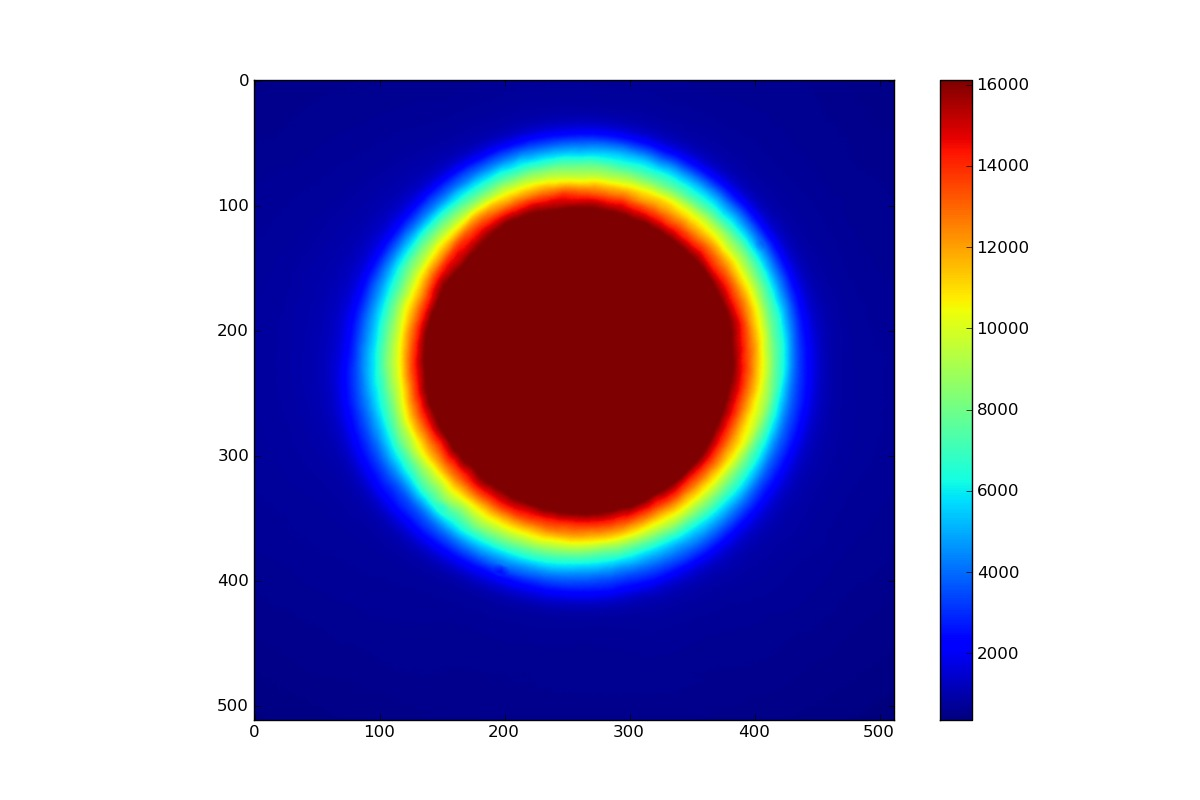
\includegraphics[height=5.9cm, trim=130 10 120 20, clip]{calib-pic}
  \pdfinput{7.4cm, trim=0 0 30 20, clip}{andor_normal_preamp5_exp30}
  \caption{{\bf left:} Image of a defocused area on a fluorescent
    plane sample. This is used for calibrating the detector. {\bf
      right:} Result of a detector calibration. The slope of the curve
    allows to convert the arbitrary analog-to-digital units into
    effective photoelectrons, the point of interception at the $y-$axis
    gives the detector read noise.}
  \label{fig:shot-noise}
\end{figure}
For the calibration of a detector, twenty images of a \cma{detector
  gain calibration} defocused fluorescent object (see left image in
\figref{fig:shot-noise}) are acquired. From the twenty images the
variance of the intensity is determined for each pixel. Then all
occurring intensities are collected into 100 bins. The average
intensity variance of each bin is then plotted against the intensity
(see right image in \figref{fig:shot-noise}). The data lie on a
straight line. From its slope we calculate the gain to convert the
arbitrary analog-to-digital units into the number of effective
photoelectrons. If the data is plotted in this unit, the slope of the
line is one, according to equation \eqref{eq:variance}. The smooth
light distribution in the input images ensures a good coverage for
each data point in the variance-intensity plot and a bit of protection
against drift.

\comment{ % this is just for copying the jpeg file
\jpginput{10cm}{calib-pic}{Image of a defocused area on a fluorescent
  plane sample.}}

To determine the quality of a detector we \cma{measuring read noise}
ensure that no light falls on the detector and create twenty dark
images.  For an ideal, noise-free detector these images would contain
zero everywhere. In a real CCD sensor the variance of the values in
the dark images reflect the readout noise $N_r$ and the mean estimates the offset. Using the calibration
gain, the readout noise can be specified as photoelectrons$/$pixel
($\unit[]{e^-/px}$).

The analysis for the right diagram in \figref{fig:shot-noise} gave a
readout noise of $\unit[5.6]{e^-/px}$. For the evaluation I used the
function \verb!cal_readnoise! of the DIPimage toolbox for Matlab
\citep{Lidke2005a}. In Appendix \ref{sec:python-readnoise-eval} I list
an alternative Python implementation of this algorithm.

The major source for readout noise is the charge amplifier. Its noise is
added uniformly to every image pixel. For readout frequencies above
\unit[1]{MHz} the readout noise increases with the square root of the
read speed \citep{Pawley2006}. Until a decade ago this limited the
readout speed of scientific CCD cameras. Then a new type of sensor was
developed --- the electron-multiplying CCD (EM-CCD) \citep{Mackay}.

This device contains an additional sequence of capacitors (denoted        \cma{electron-multiplying CCD}
multiplication registers), which are operated with a high voltage (up
to \unit[46]{V}). The field accelerates electrons and they can
generate more charge carriers by a process called impact
ionization. This is a statistical process and for every electron going
through a multiplication register, there is an average probability $p$
that it creates another electron. This probability is quite low
($p<1.3\%$) but after a sequence of 536 registers the gain
$M=(1+p)^{536}\approx 1015$ is so high, that even readout noise at \unit[17]{MHz}
readout speed can be neglected.

This amplification process consumes a lot of energy and requires an
elaborate cooling scheme of the detector chip as the gain is
temperature dependent.

Unfortunately, the statistical nature of impact ionization leads to an
uncertainty in gain and therefore introduces a \cma{excess noise
  reduces quantum efficiency} new noise source. As a gain this noise
acts multiplicatively on the signal. \cite{Robbins2003} analyzed the
amplification process and shows that the multiplicative noise, which
is also called excess noise, has the effect of halving the apparent
quantum efficiency of the detector.

Note that for very low light conditions with a minute probability to
detect more than one photon per pixel, the EM-CCD can be run with
maximum gain as a binary detector in photon counting mode. In this
mode the excess noise has no effect whatsoever; but other noise
sources become important.

\newcommand{\SNRid}{\textrm{SNR}_{id}}
\newcommand{\SNRadd}{\textrm{SNR}_{add}}
\newcommand{\SNR}{\textrm{SNR}}
\subsection{Comparison chart for detector selection}
Now I will introduce a comparison chart that I first saw in
\cite{Cameras2012}. It is based on a single equation for the
signal-to-noise ratio $\SNR$ and, if the detector parameters, such as
readout noise and quantum efficiency, are known, a quantitative
estimate of the expected quality of the data can be made.

Shot noise defines the fundamental limit for the signal-to-noise ratio
in photo detectors \citep{Sheppard2006a}. As already mentioned above,
the expected noise for a signal of $S$ photons is $\sqrt{S}$. Assuming
the contributions to a detector pixel are $S$ signal photons, perturbed
by an additional number of $I_b$ photons background light. The
signal-to-noise $\SNRid$ ratio for an ideal, noise-free detector is:
\begin{align}
  \SNRid = \frac{S}{\sqrt{S+I_b}}.
\end{align}
%FIXME wie interpretiert man das bei kleinen S, wenn gauss und poisson
%verteilung nicht gleich aus sehen?

A conventional detector with reduced quantum efficiency $Q_E\in[0,1]$
and additive, Gaussian readout noise with standard deviation $N_r$ (in
$\unit[]{e^-/px}$) can only produce a worse signal-to-noise ratio:
\begin{align}
  \SNRadd = \frac{Q_E\cdot S}{\sqrt{Q_E(S+I_b)+N_r^2}}.
\end{align}
This equation can be adapted for the electron-multiplying CCD. There,
the readout noise is reduced because of the gain $M$ but the influence
of the shot noise is doubled due to the excess noise factor
$F_n=\sqrt{2}$. \nomenclature{$F_n$}{Excess noise factor}
\begin{align}
  \SNR = \frac{Q_E\cdot S}{\sqrt{F_n^2\cdot Q_E \cdot (S+I_b) + (N_r/M)^2}} \label{eq:snr}
\end{align}
This equation permits to compare all the cameras that I can
use for my experiments. Table \ref{tab:cam-param} lists parameters
from their datasheets and the three diagrams in
\figref{fig:camera-snr} shows curves of the relative signal-to-noise
ratio $\SNR/\SNRid$ for three different amounts of background light
$I_b$.

When choosing the parameters I attached particular importance to the
noise performance, even if that comes with a loss in readout speed.

\begin{savenotes}
  \begin{table}[!htbp]
    \centering
    \begin{tabular}{l r r r r r l}
      \toprule
      camera type & $f_\textrm{read}$  & $QE$ & $N_r$ & $F_n$ & $M$ & model \\
       & [MHz] & &  [$e^-/$px] & &  &  \\
      \midrule
      back-thinned CCD & 1 & 0.95 & 5.3 & 1 & 1 &  E2V CCD97\\
      EM-CCD & 1 & 0.95 & 15.0 & $\sqrt{2}$ & 80 & E2V CCD97 \\
      EM-CCD single photon & 17 & 0.95 & 89.0 & 1 & 1000 & E2V CCD97 \\
      sCMOS global shutter& 200 &0.52 & $2.3$ & 1 & 1 & Fairchild CIS2521F\\
      sCMOS rolling shutter& 140 &0.72 & $1.3$ & 1 & 1 & Hamamatsu FL-400\\
      back-thinned sCMOS & --- &0.95 & $0.7$ & 1 & 1 & --- \footnote{Back-thinned sCMOS are not available at the time of writing.} \\
      interline CCD & 20 & 0.62 & 6.5 & 1 & 1 & Sony ICX285\\
      interline CCD & 1 & 0.62 & 2.4 & 1 & 1 & Sony ICX285\\
      \bottomrule
    \end{tabular}
    \caption{Camera parameters for the curves in \figref{fig:camera-snr}.}
    \label{tab:cam-param}
  \end{table}
\end{savenotes}

For a very large number of photons the detector with the highest
quantum efficiency $Q_E$ wins (back-thinned CCD, green line):
\begin{align}
  \lim_{S\rightarrow\infty} \frac{\SNR}{\SNRid} &=
  \frac{\sqrt{Q_E}}{F_n}. \qquad \textrm{(high light limit)}
\end{align}
For detectors with readout noise, there is a number $S_n$ of signal
photons below which the readout noise dominates:
\begin{align}
  S_n&= \frac{N_r^2}{M^2F_n^2 Q_E}-I_b.  \qquad\textrm{(photon shot noise limit)}
\end{align}
I indicate both limits in \figref{fig:camera-snr} using different line
types. The line is dotted in the region where the readout noise
dominates, followed by a thick solid line where both photon shot noise
and readout noise contribute. A thin line indicates the region where
the relative SNR is within 95\% of the high light limit and the
sensor's quantum efficiency becomes the parameter that defines the
performance.

% \gnuplotinput{camera-snr}{Comparison of signal-to-noise ratio for
%   different cameras. Dotted line for lowest light level, where $N_r$
%   is the dominant noise; thin line indicates high light region where
%   quantum efficiency and excess noise factor $F_n$ matter. }

\begin{figure}[!hbt]
  \centering
%  \svginput{1}{camera-snr-svg}
  \pdfinput{14cm}{camera-snr-svg}
  \caption{Comparison of signal-to-noise ratio for
  different cameras. Dotted line for lowest light level, where $N_r$
  is the dominant noise; thin line indicates high light region where
  quantum efficiency and excess noise factor $F_n$ matter.}
  \label{fig:camera-snr}
\end{figure}


The first thing I want to look at is the EM-CCD. For a high gain of
\cma{interpretation of EM-CCD in \figref{fig:camera-snr}} $M=20$ the
curve is horizontal and the sensor differs from the ideal detector
only in terms of a reduced apparent quantum efficiency. In a low
background environment $I_b=0.3$ the electron multiplying mode is only
advantageous for signals with less than 30 photons per pixel. For a
higher background $I_b=30$ electron multiplication does not improve
noise performance --- but note that in this mode the sensor could be
read out at a 10 times higher speed.

In a low background environment and low signal level the EM-CCD comes
very close to the ideal detector, when it is run in photon counting
mode as indicated by the blue-green line in the top left.  In this
case, however, an effect which was neglected in equation
(\ref{eq:snr}) becomes important. The impact ionization which is used
to advantage in the multiplication registers occurs with low
probability during vertical shifts of the signal and thereby adds
approximately $\unit[200]{e^-/frame}$ of spurious charge. This effect
is called clock-induced charge.

Next, I discuss the curves of the active-pixel
sensors. \cma{sCMOS in \figref{fig:camera-snr}}
The device designated as global shutter sCMOS is a sensor with five
transistors per pixel \citep{Vu2011}. Similar to a passive-pixel CCD
sensor this permits to start exposure in all pixels simultaneously,
but it has two major drawbacks. The additional two transistors cover
space that would otherwise be available as light sensitive area and
for quantitative data, a reference frame must be taken for each image,
which increases the readout noise \citep{Gamal2005,Cameras2012}.

% In his Blog Mehta reports something an Andor engineer told him:
% http://blog.mshalin.com/2012/08/global-exposure-with-scientific-cmos.html

The rolling shutter sCMOS sensor has only the minimum three
transistors per pixel and therefore a correspondingly higher quantum
efficiency. For a signal between 6 and 80 electrons per pixel this
sensor provides the best quality at 8 times higher readout speed than
the EM-CCD. Rolling shutter means that the pixel lines are read in
succession but for our prototype it is crucial that all pixels
integrate while the displays show patterns. Fortunately there is a
mode called global exposure synchronization which initiates
integration in the pixels line by line and generates a trigger output
once all pixels have started capturing light. This allows to use the
camera as a master without further effort but the camera can also be
run as a slave. In that case the only requirement is that the trigger
comes early enough ($\unit[10]{ms}$, \cite{Hamamatsu2012}) to initiate exposure in all
lines before the illumination is activated.

% 10-4 Configuring exposure time

The entry back-thinned sCMOS is only a hypothetical sensor which I
added to compare the performance of a low noise active-pixel sensor
with near perfect quantum efficiency.
\subsection{Calibration of the EM-CCD gain}
The method I presented for CCD calibration can be applied to measure
the gain $M$ and the excess noise factor $F_n$ of an EM-CCD. This
requires dark images and image sequences of the smooth intensity
distribution (from the exactly the same sample and illumination) with and without
electron multiplication gain, so that data for both cases can be
converted into detected photoelectrons.

The apparent quantum efficiency with gain is $Q_E/F_n$. Therefore the
excess noise factor can be calculated with
\begin{align}
  F_n =  N_{(1)}/N_{(M)}  
\end{align}
where $N_{(1)}$ and $N_{(M)}$ are the sums of photoelectrons in the
image without and with electron multiplication gain, respectively.

The variance for data without gain is $(\Delta I)^2_{(1)} = Q_E
\langle I \rangle$ and smaller than for data with gain, where the
variance is $(\Delta I)^2_{(M)} = Q_E F_n^2 \langle I \rangle$.

The $x-$axis in the intensity-variance plot is equal to the intensity
for gain-free data and scaled with $M$ for the amplified data.  The
gain $M$ can be calculated from both slopes $m_{(1)}=Q_E$ and $
m_{(M)}=Q_E F_n^2/M$ of the intensity-variance curves:
\begin{align}
  M = F_n^2 \frac{m_{(1)}}{m_{(M)}}.
\end{align}

In Appendix \ref{sec:basic-acquisition} I present code to
automatically measure data for this calibration. In order to cover a
large span of gains, I capture a short exposure image before each
measurement and use the longest exposure time that is possible without
overexposing the sensor.


% - effects to look out for

% - signal pickup fft of dark image to see periodic offset fluctuations

% - gain fluctuations have multiplicative influence more of a problem for scmos

% - not clear how frequent recalibration will be required


% - heating during read can lead to offset drift

% - make sure all the charge is transported out

% - light source brightness fluctuation

% - room light


% - Higher gains are possible but limit the dynamic range.

% - maximum charge handling capacity with linear response: 400000 \citep{2004e2v}


% - cic is a problem

% - thermal effects lead to generation of charge in a ccd

% - for long integration times dark current must be prevented by deep cooling (needs vacuum)


% - clock-induced charge for very fast frame rates


% % cascade II /mnt/backup/safe-with-time/torben/safed/y2009/0414
% % andor ultra ~/1114  python code for calibration and andor basic for acquisition


% - stable light source

% The top left diagram of \figref{fig:ixon} contains such a 2D
% histogram. It was obtained by conventional readout at \unit[3]{MHz} of
% our Andor IXon3 camera (head: DU-897D-CS0-\#BV). The variances are
% collected in 64 intensity bins and their averages are plotted as red
% crosses. The blue line is the result of a linear fit to the first
% $60\%$ of the red crosses. Its slope gives the real gain of the camera
% that can be used to convert ADU into photoelectrons (here
% \unit[1.32]{$e/$ADU}).

% The following figures show corresponding measurements using the EM
% readout mode with varying EM-gain. It is followed by one last
% measurement with conventional readout to verify, that the fluorophores
% did not bleach too much during the experiment.

% The camera was cooled to \unit[$-75$]{$\,^{\circ}{\rm C}$}. In order
% to prevent overexposure of the sensor a preliminary image with a short
% integration time of \unit[10]{ms} was acquired. Then, using this
% image, the integration time was for the experiment was set such that a
% maximum of \unit[10000]{ADU} would occur (in the function
% \textsf{$\sim$GetSaturationExposure}). An internal shutter in the camera
% was closed (\textsf{SetShutter}) to obtain the dark images. The process
% was automated using an Andor Solis Basic program which is listed
% below.


Table~\ref{tab:ixon-table} summarizes the calibration results. The
average of the dark images (in ADU) is given in the column
\textsf{offset}. The read noise in conventional mode is approximately
8 electrons per pixel rms. The column \textsf{mean'} (primed variable)
contains the average number of photoelectrons per pixel in the
illuminated image normalized by the integration time. The rows
\textsf{conv1} and \textsf{conv2} with conventional readout (without
EM-gain) contain approximately the same number. This proves that no
significant bleaching occurred during the experiment.

\subsection{Conclusion}

In this section I discussed how various camera sensors work. I have
explained photon shot noise, which follows from the quantum mechanical
nature of light and so far constitutes a fundamental limit of light
detection. Based on this, I explained a calibration method that helps
to evaluate camera performance and, maybe more relevant for this work,
allows to compare images that were created with different microscopes.

Since low-noise active-pixel cameras became available only late during
my project, and the first models still had some issues --- unstable
software or in the case of the Hamamatsu Orca Flash~2.8 too few
outputs for trigger signals, I designed my system for EM-CCD.  For
most experiments, however, I used an interline CCD.



% The EM-gain process introduces multiplicative noise in the signal. Its
% effect on the photoelectron statistics is the same as lowering the
% quantum efficiency of the sensor. Dividing values of the column
% \textsf{ mean'} from EM readouts by the same value from the
% conventional readout gives the \emph{excess noise factor}\todo{get
%   this right: should be $\sqrt{2}$}. Its value is smaller than one and
% describes the apparent reduction of the quantum efficiency.


% Due to a bug in the capturing process the images in the second row
% (for EM-gain 40) was overexposed and the data should not be used.  Also
% the last experiment \textsf{conv2} with conventional readout reports
% a larger gain of \unit[1.6]{e/ADU} than the first experiment
% \textsf{conv1} with gain \unit[1.3]{e/ADU}. Later we learned that one
% should allow several seconds of settling time, when changing the
% EM-gain voltage. This might explain the difference in gains, even
% though one would think that the conventional readout should be
% decoupled.






% \begin{figure}
%   \centering
%   \pdfinput{7.4cm}{andor_normal_preamp5_exp30}
%   \pdfinput{7.4cm}{andor_emgain100_preamp5_exp30}
%   \pdfinput{7.4cm}{cascade_exp400ms_normal}
%   \pdfinput{7.4cm}{cascade_exp400ms_gain3000}
%   % \includegraphics[width=7cm]{../app_cam/cascade_normal_preamp3_exp30}
%   \caption{{\bf top:} Andor IXon2 {\bf left:} Normal readout with
%     preamp 5 and \unit[1]{MHz} readout rate.  {\bf top right:} EM-gain
%     100 preamp 5. {\bf bottom:} Cascade II {\bf left:} Normal readout
%     at \unit[5]{MHz} $\textsf{mean}=\unit[254.82]{e/pixel}$. {\bf
%       right:} EM-gain 3000 at \unit[10]{MHz},
%     $\textsf{mean}=\unit[122.08]{e/pixel}$, therefore the excess noise
%     factor is 0.48.}
%   \label{fig:old-cams}
% \end{figure}

% sushi 20090414 maybe check for readout speed of cascade II and the
% excess noise factor of the andor

% check in lab book for exact specs of andor ixon2


% \subsection{sCMOS}
% pixel in
% ccd ist passiv
% cmos ist aktiv

% column parallel readout sony exmor

% exmor r additionally back illuminated (only works for small sensors)


% - typically two rolling shutters

% - global shutter increases read noise by a factor of 1.41

% - non-destructive read

% - dual amplifiers enable good low signal performance but high full
% well capacity at the same time at the expense of non-uniform gain

% \citep{Breakthrough2009}

%%% Local Variables: 
%%% mode: latex
%%% TeX-master: "kielhorn_memi"
%%% eval: (reftex-mode)
%%% eval: (flyspell-mode)
%%% End:
 
\chapter{Methods of controlling illumination patterns}
\chapter{The concept of spatio-angular microscopy}
\label{sec:concept}
\begin{summary}
  Here I introduce the spatio-angular microscope. First I explain the
  concept of its illumination system using exemplary fluorophore
  distributions, that occur in typical specimen.

  Then I describe some decisions we faced during the initial design
  phase concerning the arrangement of optical components. Furthermore,
  I position our method among known approaches of light control for
  microscopy. Of all published techniques for excitation illumination
  control, the light field microscope \citep{Levoy2006} comes closest
  to our approach.  I explain differences between both techniques and
  discuss their respective pros and cons.  I address the peculiarities
  and limitations of the hardware components in chapters
  \ref{sec:dev1} (optics) and \ref{sec:mma} (micromirror based pupil
  plane SLM).  Initially, the details would be detrimental to clarity.

  The effective use of the spatio-angular microscope, requires more
  knowledge about the specimen than a conventional or a SPIM
  microscope \citep{Huisken2004}. Ideally, the distribution of
  refractive index and fluorophores in the specimen should be
  known. If these parameters were precisely known, there would be no
  need for an image in the first place. However, while imaging a known
  specimen, sufficiently good predictions of these parameters can
  often be made. The higher the accuracy of these prognoses, the
  greater the reduction in phototoxicity will be.

  The computer-based selection of appropriate illumination masks
  requires the prediction, or at least an approximate estimation, of
  the three-dimensional distribution of light in the specimen.

  In the last part of this chapter, I describe the computational
  control loop in our spatio-angular
  microscope and touch topics of image processing.
\end{summary}
\section{Motivation}
In order to introduce the basic idea underlying the spatio-angular
microscope, I consider the distribution of excitation light in the
object of a conventional fluorescence microscope:
\figref{fig:hourglass-all}~a) schematically illustrates the side view
of the excitation beam path through objective lens and object in a
confocal microscope. A parallel beam with a circular cross-section
(this cross-section is not shown in the illustration) passes through
the lens. The lens focuses the light in its focal plane.

Between lens and focal plane the light rays form a convergent circular
cone. If refractive index variations in the object are negligible, the
light distribution below the plane of focus forms a cone as well, due
to symmetry.  Assuming a non- or weakly absorbing specimen, the energy
of the light in the circular cross-sections of the cone remains
constant\footnote{The ray-model is valid in large parts of
\figref{fig:hourglass-all}~a), but not everywhere. The Law of
Malus--Lupin states that rays and wavefronts are equivalent as long as
rays do not intersect (caustic), or (FIXME formulas?) a strong
intensity gradient occurs. Thus the ray-model is valid almost
everywhere in the cone, except for a region with a distance of a few
wavelengths to the edge, and the focus itself. While the wave-optical
treatment of these areas is possible, it is computationally much more
expensive than ray tracing. Wave-optical effects either lead to
blurring in a length scale of a few wavelengths or intensity
fluctuations due to interference. If necessary, we can use heuristics
to find an upper bound for the local intensity from ray tracing
results. For this reason we exclusively employ the ray-model in this
work.}\label{sec:ray-valid}.


The fluorescent bead (1), in the focus, would therefore be excited
significantly more than the bead (2) outside the focal plane. Also
shown is the light distribution in the intermediate image plane.

The image of the in-focus bead (1) is sharp, i.e.\ its emanating  % FIXME i need confocal here
fluorescence light is concentrated on an area as small as possible and
positioned exactly on the detection pinhole. Conversely, the image of
the out-of-focus bead (2) is blurred and its fluorescence light is
distributed over a large area.

While only a tiny proportion of the light emitted by the out-of-focus
bead contributes to the detection signal of the confocal
microscope---and therefore hardly affects the image quality, with
respect to overall phototoxicity of the full confocal system---it
would be better to prevent the excitation of the out-of-focus bead in
the first place.

\begin{figure}[!hbt] \centering \svginput{.43}{hourglass-all}
  \caption{{\bf (a)} Two fluorescent beads are illuminated by all
angles that the objective can 
deliver. The sharp image of the in-focus bead is deteriorated by
blurry fluorescence of the out-of-focus bead (2). {\bf (b)} Angular
control allows selective illumination of the in-focus bead (3), and
results in a better image on the camera. {\bf (c)} Angular control,
however, is insufficient, when an extended in-focus area is
illuminated. {\bf (d)} Then, simultaneous spatial and angular control
allows sequential excitation of the in-focus beads, while excluding
the out-of-focus bead (10).}
  \label{fig:hourglass-all}
\end{figure}

The scheme in \figref{fig:hourglass-all}~b) demonstrates how the light
cone would have to be manipulated in order to exclude the out-of-focus
bead (4). The expected fluorescence image in the intermediate image
plane then contains only information from the in-focus bead (3).

Viewed from the in-focus bead (3) the change in illumination
corresponds to a restriction of the light angles. Such control can be
exerted well through a mask in the other focal plane of the objective
lens (also denoted back focal plane or pupil plane).

Thus it is useful and possible to equip a confocal microscope with
angular control. However, in our project we set out to to build a wide
field microscope in order to benefit from the speed and quantum
efficiency of modern cameras.

I now turn to the task of bringing angular control to the wide field
microscope. \figref{fig:hourglass-all}~c) shows a configuration of the
specimen with two in-focus beads (5) and (6), and one out-of-focus
bead (7).  The angular illumination control is ineffective for this
arrangement of beads.  If both in-focus beads, (5) and (6), are
exposed simultaneously, i.e.\ an extended light source illuminates the
entire field, then the out-of-focus bead (7) is always excited.

Only by separate illumination of the in-focus beads (8) and (9), as
shown in \figref{fig:hourglass-all}~d), angular control regains its
function. For this reason a wide field system with angular control,
using a mask in the pupil, requires an additional mask conjugate to
the field.  Therefore, we call our method spatio-angular
microscopy. ``Spatial'' refers to the illumination control in the
field and ``angular'' refers to the control in the pupil plane.

% FIXME 2012 khodjakov schilling

\begin{figure}[!hbt] \centering \svginput{1.5}{memi-simple}
  \caption{Simplified schematic of the illumination system in our
spatio-angular microscope. A homogeneous extended light source
delivers light from the left. It is imaged by lenses $L_1$ and $L_2$
into the intermediate image $F'$. Then the tubelens $L_3$ and the
objective $L_4$ form an image of $F'$ in the sample plane $F$. We use
two spatial light modulators (SLM) to control the spatial and angular
light distribution in the specimen---the focal plane SLM in F', and
the pupil plane SLM in P'.}
  \label{fig:memi-simple}
\end{figure}

\figref{fig:memi-simple} shows the optical path through our prototype
in a simplified form.  From the left side, an extended light source
illuminates the system. A sequence of telecentric lenses $L_1$, $L_2$,
$L_3$ and the objective lens $L_4$ image the light source from F''
into the front focal plane (indicated by F, for field). The etendue
(see page \pageref{sec:etendue} for its definition) of the light
source must be large enough to simultaneously fill both, the pupil P
as well as the field F.

In each of the two planes P' and F' we place a spatial light modulator
(SLM) that allows to control the intensity of the transmitted light.

Looking at the scheme in \figref{fig:memi-simple}, one might argue
that we could save a lens, if we placed the pupil plane SLM into P
instead of P'. There are three reasons why this is neither possible,
nor beneficial: First, the pupil of modern high-performance objective
lenses is typically not accessible. Second, the detection path for
fluorescent light should contain as few optical components as possible
and we can definitely not afford it to be blocked by a SLM.  Third,
the two masks induce non-linear, and therefore difficult to predict,
filtering of spatial frequencies. An analysis requires consideration
of partial spatial coherence, but it should be clear (FIXME) that only
the downstream\footnote{Downstream regarding the propagation direction
  of the excitation light.} SLM will always deliver a good image,
mostly independent of the state of the SLM upstream.

Considering the fact that the image of the focal plane SLM is most
important to us, we decided to place it downstream of the pupil plane
SLM. The focal plane SLM may disturb the image of the pupil plane SLM
in P, but we can always produce very fine, high-contrast structures in
the sample F.

The abiltity to achieve high resolution in the field is the main
difference between our approach and Levoys light field microscope.  In
the light field microscope, the density of the microlenses noticeably
limits the resolution. As opposed to our system, the light field
microscope allows to control the angle of incidence in all field
positions independently.  But, additionally to the reduced focal plane
resolution, this requires a single high-resolution SLM with a
comparatively low refresh rate. We use two small SLMs, which can each
achieve \unit[1]{kHz} frame rate and enable interesting experiments,
e.g.\ optogenetic control of neuron activities.

Furthermore, structured illumination with high resolution patterns
allows us to circumvent the missing cone problem of the widefield
microscope.  Later I will show that depth discrimination improves with
higher resolution patterns (FIXME ref).
\section{An imaging protocol with spatio-angular illumination control}
\subsection{Description of an exemplary biological specimen} 
I now refer to the \celegans\ test sample for phototoxicity that I
introduced in section \ref{sec:intro-phototoxicity}. So far I did not
reach the point of being able to image the development of a real
embryo. Key problems are the low light throughput of the illumination
system and the length of time necessary to update images on the focal
plane display. Nevertheless, I always kept this example in mind while
I was developing the control software for our microscope.

During the first few hours, the embryo develops confined within the
constant volume of its egg, which has an ellipsoidal shape, extends 40
to 60 microns and can be readily observed using a $63\times$ objective
lens. Cell divisions occur every few minutes.  During development the
nuclei get smaller and more dense. In order to track the fate of all
individual cells it is sufficient, to capture one stack per minute
with 41 layers and a $z-$step of 1~micron.
\subsection{Preparation of living embryo samples} 
For an experiment a hermaphrodite worm is cut and the embryos are
placed on an agarose pad, so that they stay immobile during
imaging. This procedure is explained\footnote{Note that
  \cite{Murray2006} describes an improvement of this protocol that
  prevents squeezing the embryos too much.} in \cite{Hope1999}. Of
these embryos, the experimentor chooses a young specimen, that has not
yet divided. We avoid to use fluorescence excitation for this step.
The undivided embryos can be distinguished using the less phototoxic
differential interference contrast (DIC) imaging mode.

\subsection{Sectioning through structured illumination} 
To get an estimate of the initial distribution of the fluorophores in
the embryo I obtain the very first stack with structured illumination
and no angular control. I use this method to avoid the missing cone
problem of the widefield microscope. Perhaps for our particular task
of finding the position of one nucleus within the egg, widefield
images would be just sufficient.  However, for our spatio-angular
method, knowledge about the fluorophore distribution is very important
and therefore we built our microscope such that we can obtain optical
sections.

We compared conventional structured illumination using max$-$min
(FIXME) reconstruction with laser and LED illumination. Although LED
illumination resulted in excellent optical sections, the
reconstruction of laser illuminated images contained artifacts.

% {\color{red} - (FIXME muss das vielleicht in appendix?) In einem
% ersten Entwicklungsschritt, bevor InVision uns den Prototyp fuer das
% spatio-angulare Mikroskop zur Verfuegung stellte, setzten wir einen
% SLM in die Zwischenbildebene. Auf dem SLM wurden vier Streifenmuster
% angezeigt und Wir verglichen einen 70mW 473nm DPSS laser mit 470nm LED
% Beleuchtung (CoolLED).}

Therefore, we decided to implement HiLo (see Appendix FIXME). With
this algorithm, we obtain artifact-free optical sections, regardless
of the illumination source. As another advantage the HiLo method
increases acquisition speed, because only two raw images per slice are
necessary.


% {\color{red} wir haben artefakte in der max-min rekonstruktion
% beobachtet, wenn wir ein grobes streifenmuster (8 forthdd slm pixel
% periode) mit laser beleuchtet haben

%      - irgendwann hat rainer das erklaert aber ich kann mich nicht
% mehr dran erinnern aber es waere cool, wenn ich die story bringen
% koennte
     
% - grobes gitter heisst im amplitudenbild: einige ordnungen (nicht nur
% 3) gehen durch die bfp

%      - irgendwie kam es dadurch im intensitaetsbild zu einigen hoehere
% ordnungstermen

%      - bei LED (extended source) werden die weggemittelt, bei laser
% nicht

%        - ein bisschen kopfzerbrechen bereitet mir noch der bias

%        - im paper habe ich das nicht verstanden [2011 mertz Optically
% sectioned in vivo imaging with speckle illumination HiLo microscopy]

%        - aber ich habe ihr java imagej plugin decompiliert bekommen
% und koennte versuchen ihre implementierung zu verstehen (andererseits
% ist mir das jetzt ziemlich egal)

%        - unter equation 10: The first two terms are variance
% contributions of shot noise. Filtering has the effect of reducing
% noise variance and is taken into account with the integral term. This
% bias must thus be subtracted from $\sigma^2$ prior to the evaluation
% of C. We have also not considered the effects of pixelation in the CCD
% camera. If the pixel size is non-negligible ..  }

\subsection{Computer model for the integration of a priori knowledge
about the biological events} 
Given an initial measurement of the fluorophore distribution of the
embryo, I employ a computational algorithm to find good illumination
conditions for subsequent stack acquisitions. An important requirement
is that the computer can estimate, which areas of the sample should be
protected from illumination.

For our test system, the \celegans\ embryo, it is a promising approach
to represent its three-dimensional fluorophore distribution by a
simple model: Spheres encompassing the nuclei, indicate regions with
fluorophores. When in focus, the spheres are the source of useful,
informative fluorescence signal, but should be protected against
exposure when out of focus.

As I mentioned earlier, there are also unused histones with
fluorophores outside of the nuclei. The images reveal that they occur
in the cytoplasm at a much lower concentration than in the
nuclei. Fluorophores in the cytoplasm have a smaller phototoxic
effect, because any radicals they produce are much less likely to
reach the DNA and therefore inflict substantially less damage.  In the
following my goal is to protect only out-of-focus nuclei from
exposure. The regions in between are used to bring the light in.


During observation, the nuclei, i.e.\ the centers of the spheres, move
slowly within the embryo. For small periods of time we can describe
this movement using a vector field of growth velocities.

A cell division announces itself by a change of the fluorophore
distribution of the nucleus due to chromatin condensation and spindle
formation. Therefore, whenever the computer detects such changes in
the images, in one of the following time steps an additional sphere
should be introduced to account for the new daughter cell.

So far I have implemented a simple algorithm, to convert a time series
of image volumes from a confocal microscope into a sphere model
\citep{Santella2010}.  One of our project partners (Jean-Yves Tinevez,
http://fiji.sc/wiki/index.php/TrackMate) developed a more
sophisticated plug-in for ImageJ, that provides the lineage tree and
snapshots of the developing cells (see \figref{fig:trackmate}).
\begin{figure}[!hbt] \centering
  \pdfinput{6cm}{TrackMate_Celegans_lineage}
  % trim=left bottom right top
  \qquad
  \includegraphics[trim=25cm 0cm 84cm 87cm, clip, height=5cm]{TrackMate_Celegans_lineage_vector}
  \caption{ A detail of a lineage tree visualized in TrackScheme. An
    image of each nucleus is shown in each time step. Note the
    elongated structure of the nucleus before the cell division
    event.}
  \label{fig:trackmate}
\end{figure} Before our microscope can be used for our biological
problem, the computer model has to be extended so that it reliably
tracks the movement of nuclei.  Overlooking any nucleus would prevent
this nucleus from being imaged in later acquisitions and would be a
setback for the experiment.  Estimating the vector field of growth
velocities helps to track nuclei more robustly and allows to predict
their positions for the next exposure.

Currently we have not implemented programs that would fulfill the
requirements for imaging a developing embryo.  However, in the
following text I assume that the described position predictions were
available and I discuss how I determine masks for the focal plane and
pupil plane SLM.

\cite{Murray2006}

TODO FIXME Bernhard Kauslers work is nice
\verb!http://archiv.ub.uni-heidelberg.de/volltextserver/11820/1/thesis_fkaster.pdf!
Live-cell microscopy image analysis for the study of zebrafish embryogenesis
\verb!http://hci.iwr.uni-heidelberg.de/publications/mip/techrep/kausler_12_discrete.pdf!
A Discrete Chain Graph Model for
  3d+t Cell Tracking with High
    Misdetection Robustness

(FIXME read this)


\subsection{Illumination optimization by means of raytracing} 
I now discuss a method to find both SLM masks for image acquisitions
with minimal phototoxicity. First I define a mask for the focal plane
SLM:

From the predicted arrangement of spheres we select in-focus nuclei by
intersecting the model with a planar surface. I then define focal
plane SLM masks to selectively illuminate each of the in-focus nuclei,
by drawing a bright disk in the appropriate position.

Based on such a mask, we can determine which angles can illuminate the
in-focus target nucleus, without exposing out-of-focus nuclei.

As I already explained at the beginning of this chapter on page
\pageref{sec:ray-valid}, ray-optical theory suffices to describe the
light distribution within the sample.

I connect the periphery of an out-of-focus nucleus with a point inside
the in-focus target. This defines a circular cone of rays, that are
propagated through the objective lens. Their intersection with the
pupil plane results in a figure that still very much resembles a
circle---I found that already seven rays lead to good representation
of its perimeter.  An algorithm computes these figures for every
out-of-focus nucleus and for a few in-focus targets points within the
bright areas of the focal plane pattern. In this manner I construct
the desired mask for the pupil plane SLM.

In order to trace the rays into the pupil, I need the design
parameters of the objective lens (vertex position, curvature and
material for all surfaces). Unfortunately, these rarely are publicly
available for high-performance objective lenses. Nevertheless, in
chapter (FIXME) I use a simpler model of the objective lens, that
requires only three parameters: focal length, refractive index of the
immersion medium and numerical aperture. These are always known.

Additionally, I have adapted the model for non-index-matched embedding
of the specimen. This problem occurs when the embryo is illuminated
with an oil immersion objective, using HILO (FIXME ref). It should be
noted, however, that good image quality of the embryo can only be
achieved with an objective lens that has the same immersion index as
the embryo. Otherwise data from 20 microns within the sample will be
severely deteriorated by spherical aberrations.

\chapter{Device 1: prototype for spatio-angular illumination}


\begin{figure}[!htbp]
  \centering
  \svginput{2}{memi-real}
  \caption{Schematic of the light path through our microscope. Laser
    light enters from the lower left, is scrambled and homogenized to
    illuminate the full MMA and LCoS. $F$ is the field plane in the
    sample and its primed versions are conjugated planes. $P$ is the
    pupil of the objective. $B_0$ and $B_1$ are adjustable circular
    apertures. PBS is a polarizing beam splitter. DBS is a dichromatic
    beam splitter.}
  \label{fig:memi-real}
\end{figure}

\begin{figure}[!htbp]
   \centering
   \svginput{2}{memi-sketch}
   \caption{Schematic of the lenses in the MEMI system and their focal
     lengths. The focal length $f_\textrm{TL}$ of the tube lens can be
     varied. This allows to scale the second intermediate image
     $r''_\textrm{MMA}$ of the micro mirror array to fit the back
     focal plane of different objectives. Dimensions in mm.}
   \label{fig:memi-sketch}
 \end{figure}

\jpginput{14cm}{setup-photo-blueprint}{The wide field epi-fluorescence
  microscope with attached illumination head. The positions of the two
  spatial light modulators (Micro mirror array (MMA) and liquid
  crystal on silicon display (LCoS)) are indicated. Drawing by Josef
  Wenisch (In-Vision, Austria).}

% \imagw{14cm}{mma}{{\bf left:} Scanning electron microscope image of
%   the micro-mirror array (MMA).  The pixel pitch of the device is
%   \unit[0.016]{mm}. The hinges for the tilt movement and the
%   electrodes are clearly visible. {\bf middle:} Optical reflective
%   microscope image of the MMA. {\bf right:} exaggerated rendering of
%   how a 8x8 checker board pattern would be displayed on the
%   device. Electron and optical micrograph by Fraunhofer IPMS Dresden
%   (Germany)}

% \begin{figure}[!hbt]
%   \centering
%   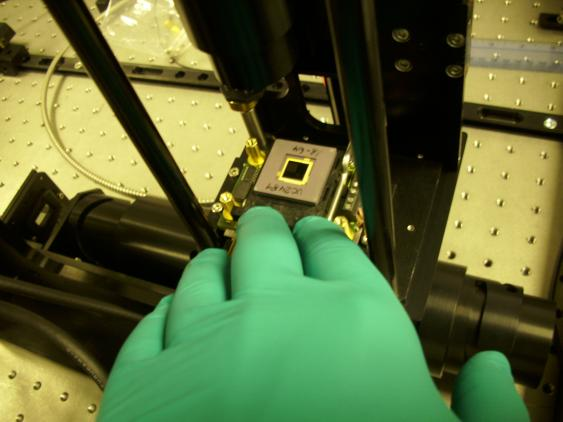
\includegraphics[width=7cm]{mma-plain}
%   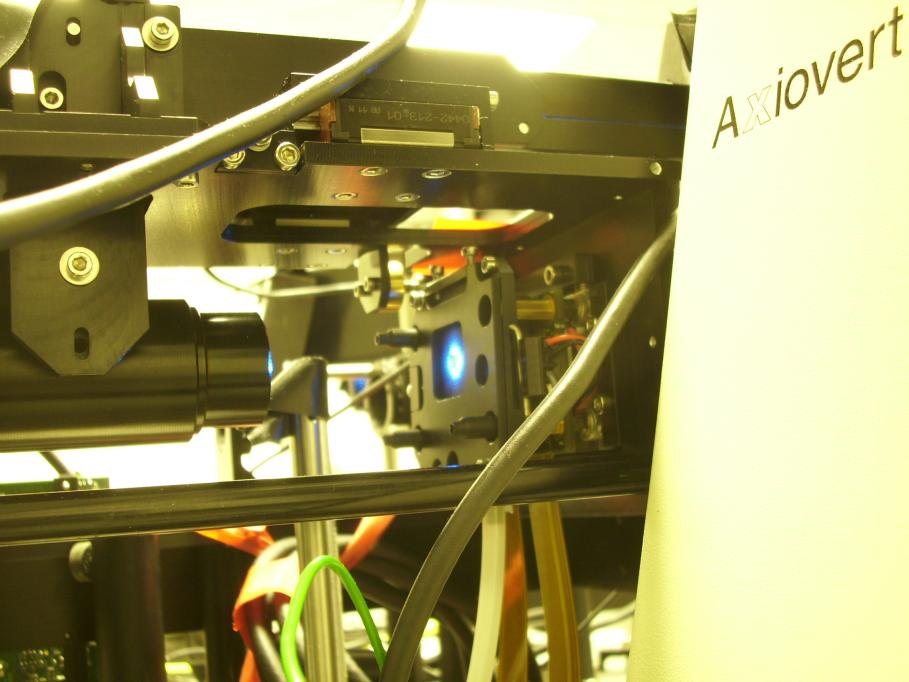
\includegraphics[width=7cm]{mma-ill}
%   \caption{{\bf left:} Micro mirror array chip during installation of
%     the optics. {\bf right:}~Illuminated micro mirror array in the
%     aligned system.}
%   \label{fig:mma-closeup}
% \end{figure}

\chapter{optimization of the spatio-angular illumination patterns}
\label{sec:optimization}
\chapter{mma as an intensity modulator}
\label{sec:mma}
\include{device2}
\chapter{experimental results with spatio-angular microscope (device 1)}
\label{sec:results}
\chapter{discussion}
\label{sec:discussion}
- zuerst habe ich dvi lcos mit mma verbaut, das hat leider nur
  gelegntlich funktioniert

- urspruenglich war geplant folgendes system einzusetzen: Biological
  applications of an LCoS-based programmable array microscope (PAM)

- dann habe ich usb lcos eingesetzt, damit geht es immer, ist aber
  langsamer und deutlich weniger nuetzlich zum experimentieren

- ausserdem ist die ettendue des beleuchtungssystems arg
  eingeschraenkt mit einem 63x objektiv (NA=1.47) wird nur ein feld
  mit 40 um durchmesser beleuchtet

- deshalb untersuchten wir einen anderen weg zur kontrasterzeugung und
  lernten dabei dass ein interferometrischer ansatz sehr wohl geeignet
  ist, die ettendue zu erhoehen

  - einschraenkungen in der realisierbaren optik (freier durchmesser
    der nomarski prismen) fuehrte zu nicht ganz ueberzeugenden bildern

  - ein piston mma wuerde zu deutlich besseren ergebnisse fuehren

- ein weiterer ansatz fuer spatio-angular beleuchtung wurde mit einer
  holographischen methode verfolgt

  - dabei lernten wir dass die qualitaet des verwendeten
    phasenmodulators zu wuenschen uebrig laesst

  - einfacherer ansatz mit nur einem display, erfordert daher weniger
    optik und elektronik

  - loest jedoch nicht das problem geringer ettendue (die moegliche
    ettendue muss ich mir genauer ueberlegen, sie haengt mit der
    anzahl der pixel des displays und den grating konstanten zusammen,
    die dargestellt werden koennen, da das system off-axis betrieben
    werden muss, wird die ettendue geviertelt)

- Im Nachhinein muss man sagen, dass es Zielfuehrender gewesen
    waere, und unsere Aufgabe erheblich vereinfacht haette, wenn wir
    beide SLM vom gleichen Typ verwendet haetten. Es handelte sich
    aber um einen Prototypen und er war in den ersten Jahr des
    Projektes noch nicht verfuegbar. Das Projekt wird von Pasteur und
    Fraunhofer, diesmal unter Verwendung zweier ihrere SLM,
    weitergefuehrt. 

  - Leider wird dieser Ansatz unsereserachtens nicht das wesentliche
    Problem der kleinen Ettendue bereinigen und der neue Prototyp wird
    noch immer nicht die interessantesten Experimente erlauben. Es ist
    ganz einfach so, dass es einfacher waere, ein biologisch
    Relevantes Experiment zu designen, wenn das Beleuchtungssystem
    auch die volle Ettendue heutiger Mikroskopobjektive ausschoepft.

- kameras sind zur zeit an einem wendepunkt. vermutlich wuerde man
  heutzutage eine sCMOS benutzen, dann sollte man aber auf die
  triggereigenschaften achten

- arduino war nuetzlich um die elektronische triggerung ohne grossen
  aufwand umzusetzen (der hauptaufwand war oft nicht die
  zeitsteuerung, sondern eine ordentliche galvanische entkopplung der
  displays, die ist auch wichtig)

  - da unterscheiden sich die hersteller ohnehin sehr stark, bei dem
    dvi display war es erforderlich, testpunkte vom board abzugreifen
    und ueber adum zu entkoppeln, bei neueren varianten des usb boards
    kann man mittlerweile einfach einen stecker anstecken

- man kann relativ viel aufwand bei der rekonstruktion von optisch
  geschnittenen bildern betreiben, fuer das reale problem ist die
  vermeidung von artefakten dann oft doch nicht so wichtig (z.b. beads
  oder nuklei lokalisieren)

- transmission ist nicht ausreichend um wuermer zu untersuchen  

- vergleiche die folgenden displays:

  - holoeye (erwaehne triggerversuche, kalibrationsmessungen von
    uebertragungsfunktion und interpixel cross talk, hamamatsu)

  - forthdd (frage sie vielleicht, ob sie mir im nachhinein doch noch
    information geben)

  - ti dmd (sehr gute dokumentation, sehr viele funktionen; gut waere,
    wenn ich ein programm auf dem lokalen arm prozessor laufen lassen
    koennte, was die vollen 4000fps aus runlength (oder irgendwie
    komprimierten) daten vom usb aus erzeugen koennte

    - deflection angle defines f/\# number of projection lens and
      therefore etendue, for good contrast f/\# shouldn't be smaller
      than f/2.8

  - mma (naja)

- hilo ist nicht unbedingt notwendig, ziemlich kompliziert und brauch
  fudge factor

\chapter{outlook}
\label{sec:outlook}
- den algorithmus zur beleuchtungsoptimierung kann man noch deutlich
  verbessern

  - gleichzeitige beleuchtung mehrerer nuklei

  - andere objektstrukturen (z.b. zylinder, axone)

    - 2010 hermann cuntz: One Rule to Grow Them All: A General Theory
      of Neuronal Branching and Its Practical Application

      - modell wie neuronen wachsen um axon oder dendritendichte
        vorherzusagen

  - voxels05\_final

- eine genaue analyse einiger probleme mit wellenoptischer partiell
  kohaerenter theorie steht noch aus und waere interessant (nach
  wichtigkeit)

  - partiell kohaerente simulation des mma im schlierenoptischen system

    - sind graulevel vorteilhaft?

    - wuerde ein mma, bei dem alle spiegel in dieselbe richtung kippen
      die ettendue verdoppeln?

  - partiell kohaerente simulation des mma im shearing
    interferometrischen system

    - was ist die maximale ettendue eines wollaston prismas?

  - holographie methode mit extended source

  - Denkbar waere auch ein scannendes konfokales Mikroskop, dass an
    die Beleuchtungswinkel an jedem Punkt kontrolliert (siehe
    fig:hourglass-all-b).  Bisher wurden in der Literatur nur Systeme
    beschrieben, die die Phase des Beleuchtungslicht in der Pupille
    aendern (FIXME ref). Eine Adaption dieser Systeme zu einem
    spatio-angularen ist naheliegend und ich schlage vor, derartige
    Systeme auch untersucht werden sollten. Die Kombination von CLEM,
    einem Ringdetektor (vielleicht mit UZI) koennte die Bildgebung im
    Inneren lebender Organe (z.B. Gehirn) verbessern.


%\include{app_term}
\bibliographystyle{abbrvnat}
\bibliography{literature}
%\bibliography{../All}
\end{document}


%%% Local Variables: 
%%% mode: latex
%%% TeX-master: t
%%% End: 
